\chapter{Experimental Results and Discussion}

\textit{In this chapter, the different components of the proof of concept explained in \cref{chap:method} are tested and the results are shown. These results are discussed afterward. First, the experimental setups are outlined that facilitated the results in \cref{sec:results-experimental setup}. Afterwards the \ac{SHS} components are tested individually in \cref{sec:results-SHS}. Hereafter the whole SHS-PF with activity recognition is treated in \cref{sec:results-SHSPF}.}

\section{Experimental Setups}
\label{sec:results-experimental setup}
In order to determine the performance of the Step and Heading System Particle Filter and its components, different experiments were devised. For some components within the system, tests were performed outdoors, while others were confined to indoors. \par 

\subsection{Outdoor Experiments}
The step detection and step length estimation components are tested using a combination of data made available online under an open license and experimental data collected. The online data used for step detection and length estimation derive from the research upon which the individual methods are based, thus the data of \citet{Salvi2018} and \citet{Vezocnik2019}. The advantage of using online data is that it allows testing of techniques using the data from multiple test subjects holding a smartphone in multiple carrying modes, without having to perform extensive experiments.  \par 

The experimental data was collected personally, using an available smartwatch and smartphone. The step detection and step length estimation experiments for gathering experimental data were performed outdoors using only a smartphone carried in front, with the screen point up carrying mode, as in \cref{fig:experiment_carrying_position}. The experiments were performed outdoors since the location does not affect accelerometer readings and outdoor testing allows for long straight walking distances, which are also easily measured from satellite images.\par 

For step detection, accelerometer measurements were recorded using different carrying modes while counting the number of steps. For step length estimation, known distances were walked and compared with the total distance estimated using the devised method. Further details on the experiments can be found in their respective sections, \cref{sec:results-step_detection} and \cref{sec:results-step_length_estimation}.    \par

\subsection{Indoor Experiments}
\label{sec:results-experi_setup-indoor_experi}
The whole indoor localization system experiments were performed at the residential property introduced in \cref{sec:method-particle_filter}. The tests consisted of walking around indoors with an android smartphone in hand and recording the \ac{IMU} signals in the phone through a dedicated Android app. In addition, a smartwatch was worn around the wrist of the hand that was not holding the smartphone. This hand was used to open and close doors. The opening of doors was also indicated manually through the app on the smartphone, which had a button to record timestamps when pressed.\par 

In addition to recording \ac{IMU} data from both smartphone and smartwatch while the path was being walked, the trials were also being filmed from a breast pocket by another device. The video recordings are used to get a rough estimate of the path walked during the trial. This was done by replaying the video and pausing it at one-second intervals. At the paused moments, the approximate position was manually indicating on the map of the experiment location. The map position and time elapsed since the start of the trial were recorded. The resulting trajectory can be used to give a rough performance indication of the indoor localization method. The full experimental process can be found in \cref{appendix:shs_experiment}. \par

A total of 6 trials were walked by one test subject, each trial with a different walked path than the previous trials. The same person that generated the experimental data for the step detection and step length estimation experiments was also used for the indoor orientation and localization experiments.\par 

\section[SHS Testing]{Step and Heading System Testing}
\label{sec:results-SHS}
The individual components of the \acl{SHS} can be tested and evaluated using various data sources and experiments. Within this section, each component will be treated. At the end of the section, a qualitative evaluation of the \ac{SHS} within the indoor experiments will be analyzed. 

\subsection{Step Detection Testing}
\label{sec:results-step_detection}
The step detection method presented in \cref{sec:meth - step detection} is tested on both online and experimental data. In this section, first an overview of the relevant online data will be given, followed by several different metrics with which the performance of the step detection method from \cref{sec:meth - step detection} is evaluated. 


\subsubsection{Online Data}
\citet{Salvi2018} have released the raw accelerometer data used for their step detection algorithm under an open license. The raw data consists of sampling time and three raw accelerometer axis signals. In addition, it indicates when a new step has been detected by a ground truth device used within the research. The ground truth device consisted of sensors placed in the soles of the test subject's shoes. This device could measure when the foot applied pressure to the sole of the shoe, indicating contact with the floor, hence when a step is taken. The dataset contains data of two users carrying the phones in different carrying modes. These are in an armband, back pocket, bag, front pocket, hand, and neck pouch. This dataset provides the opportunity to assess the performance of different step detection techniques, by comparing detections with the ground truth.\par

\subsubsection{Step Counting}

The step detection implementation outlined in \cref{sec:meth - step detection} was applied to the dataset of the researchers. The total number of steps taken was calculated and compared with the amount indicated by the ground truth. The results can be found in  \cref{fig:sd_abs_comparison} and \cref{fig:sd_percent_comparison}. \cref{fig:sd_abs_comparison} compares the number of steps detected and actually taken, while \cref{fig:sd_percent_comparison}  shows the corresponding percentage error, where positive percent error indicates over-counting, while negative under-counting. \par 

In addition to the data made available online, experimental data was gathered outdoors in which a test subject walked exactly 60 steps in a straight line while having a smartphone in 3 different carrying modes, back pocket, front pocket, and in hand. Two trials per carrying mode were performed. The steps were counted manually. The percentage error from the ground truth can be seen in \cref{fig:202009291013step_counting_error_of_60_steps}.

The results using the opensource data of \citet{Salvi2018} indicate that the step detection implementation performs well for most carrying modes. Many of the carrying modes have a percentage error close to 5\% or less. The results of the step detection applied to experimental data show similar results as with the opensource for smartphone in hand carrying mode, with a slightly larger error in the front pocket carrying mode.\par 

In both the opensource and experimental data, bad step detection performance in the back pocket carrying mode was found. Researchers attribute the bad detection in the back pocket to the pocket being loose and allowing the phone to rebound when a step was taken \cite{Salvi2018}. This would introduce nefarious components in the accelerometer signal, leading to false positives. \citet{Brajdic2013} encountered similar problems with this carrying position, hypothesizing that the relaxing of the gluteus maximus during locomotion could influence the acceleration trace.

	\begin{figure}[htbp]
		\centering
		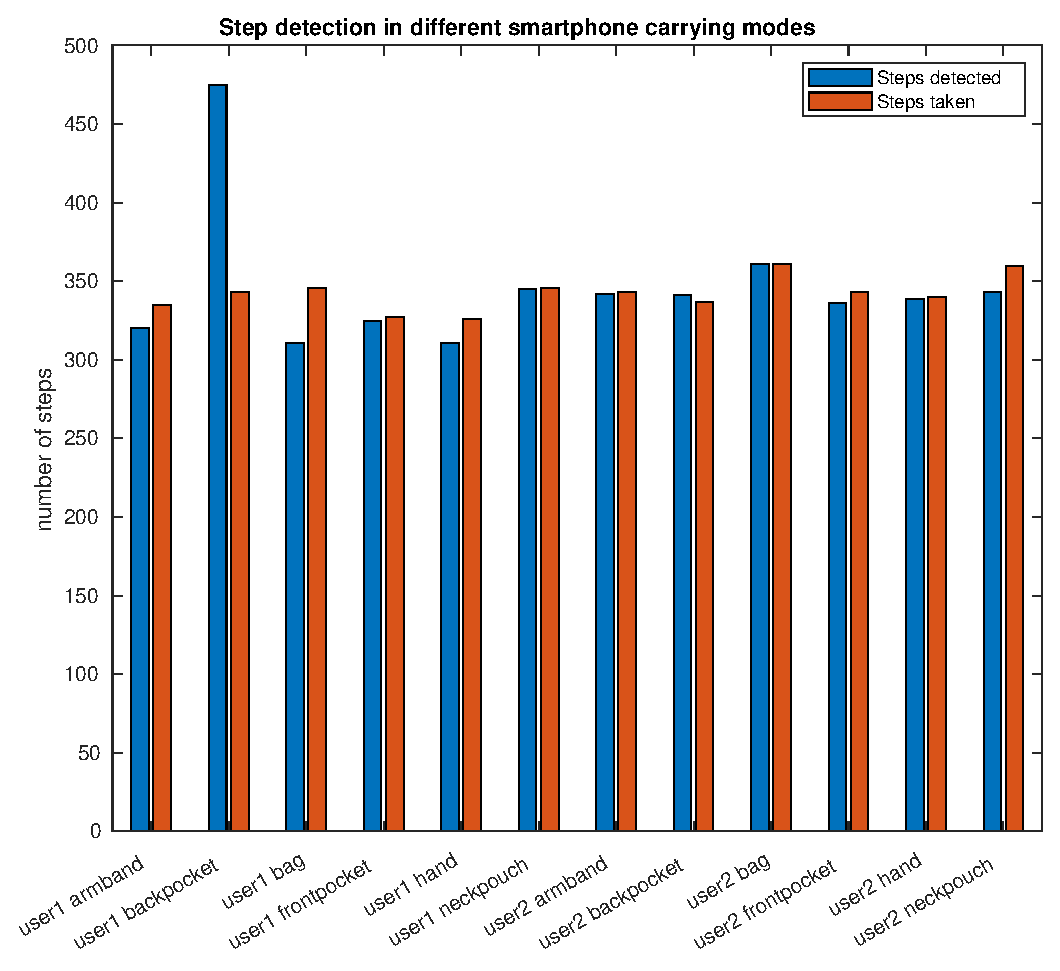
\includegraphics[width=0.7\linewidth]{images/20201127_1516_Step_detection_in_different_smartphone_carrying_modes}
		
		\caption{Absolute number of steps detected using method in \cref{sec:meth - step detection} on \citet{Brajdic2013} dataset.}
		\label{fig:sd_abs_comparison}
	\end{figure}
	\begin{figure}[H]
		\centering
		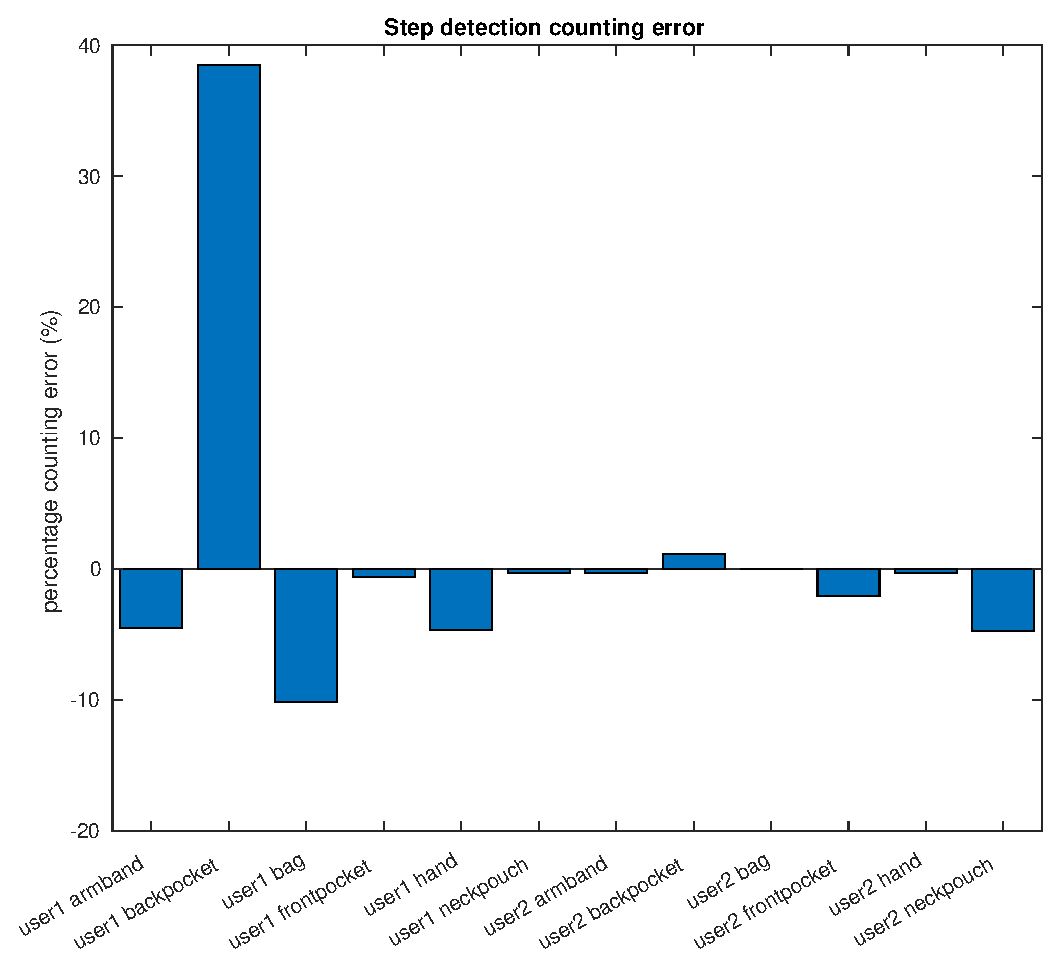
\includegraphics[width=0.7\linewidth]{images/20201127_1520_Step_detection_counting_error}
		\setlength{\belowcaptionskip}{-10pt}
		\caption{Percentage error step detections from steps taken using method in \cref{sec:meth - step detection}. }
		\label{fig:sd_percent_comparison}
	\end{figure}

%	\caption[Step detection comparison]{Comparison between \citet{Salvi2018} step detection algorithm, \cref{algo:step_detect} and ground truth for different carrying modes.}
%	\label{fig:sd_comparison}
\begin{figure}[H]
	\centering
	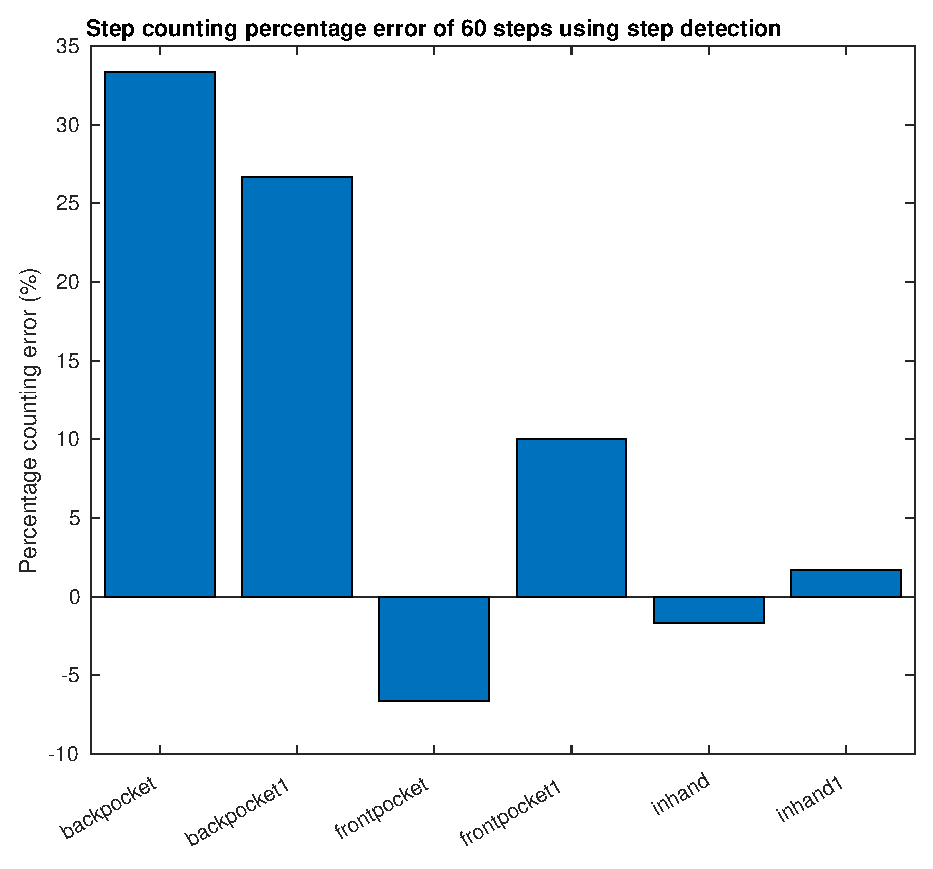
\includegraphics[width=0.7\linewidth]{images/20201127_1640_Step_counting_percentage_error_of_60_steps_using_step_detection}
	\setlength{\belowcaptionskip}{-20pt}
	\caption{Experimental data step counting using method in \cref{sec:meth - step detection} on \citet{Brajdic2013} dataset.}
	\label{fig:202009291013step_counting_error_of_60_steps}
\end{figure}

\subsubsection{Time Difference between Detection and Ground Truth Step}

For a \ac{SHS} it is not enough for the number of steps detected to be accurate, but also the time when a step actually occurs. Detecting a step, combined with the heading orientation at that moment, determines the direction of the step. It is therefore preferable for a detection to be as close as possible to when a step actually occurs, with no other detections in the vicinity. \par
Using the \citet{Salvi2018} data with ground truth step detection, the time difference between a step detection and its closest ground truth point was calculated per trial. The mean and standard deviation of the time difference for each carrying mode was calculated, shown in \cref{fig:202011130914smallest_diff_to_gt_1}. 

\begin{figure}[H]
	\centering
	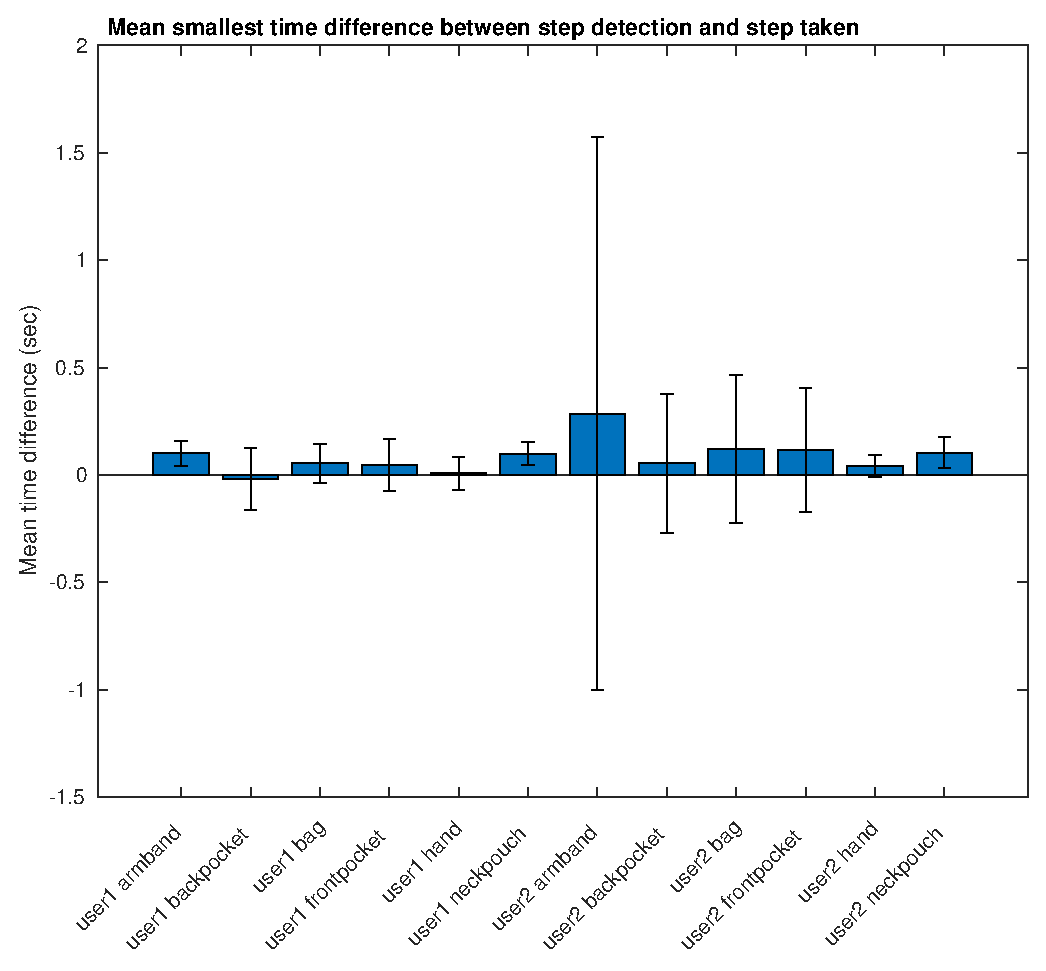
\includegraphics[width=0.7\linewidth]{images/20201127_1607_Mean_smallest_time_difference_between_step_detection_and_step_taken}
	\caption{Mean and standard deviation of the smallest time different between step detection and step occurrence using method in \cref{sec:meth - step detection} on \citet{Brajdic2013} dataset . A positive difference indicates detection before step occurrence and negative after occurrence}
	\label{fig:202011130914smallest_diff_to_gt_1}.
\end{figure}

The results show that most detections are within 0.1 seconds from the closest ground truth point. The best performing carrying mode is in hand. The large standard deviations for "user2 armband" is caused by the step detection methods having already counted multiple steps before the ground truth device has registered any. The low time difference for the back pocket carrying mode supports the hypothesis that double counting is occurring close to the step since the time differences to the actual steps are small.

\subsubsection{Unique Step Detection}

One problem with the time difference between detections and steps taken is that two subsequent detections may have the same ground truth point as the nearest point, indicating that there is no unique detection of the step occurring. \par 

An approach to determining unique step detection performance was fashioned. Since it is unrealistic to expect the step detection to be at the exact time an actual step occurs, intervals are defined around ground truth step where if a step is detected once within the interval using the method in \cref{sec:meth - step detection}, the detection counts as a unique step. If in this interval two steps are detected, no unique step is indicated. The time interval is increased iteratively in an attempt to find the highest unique step counts. The results for each user and carrying mode can be found in \cref{fig:sd_tp_fp_comparison}. 

\begin{figure}[H]
	\centering
	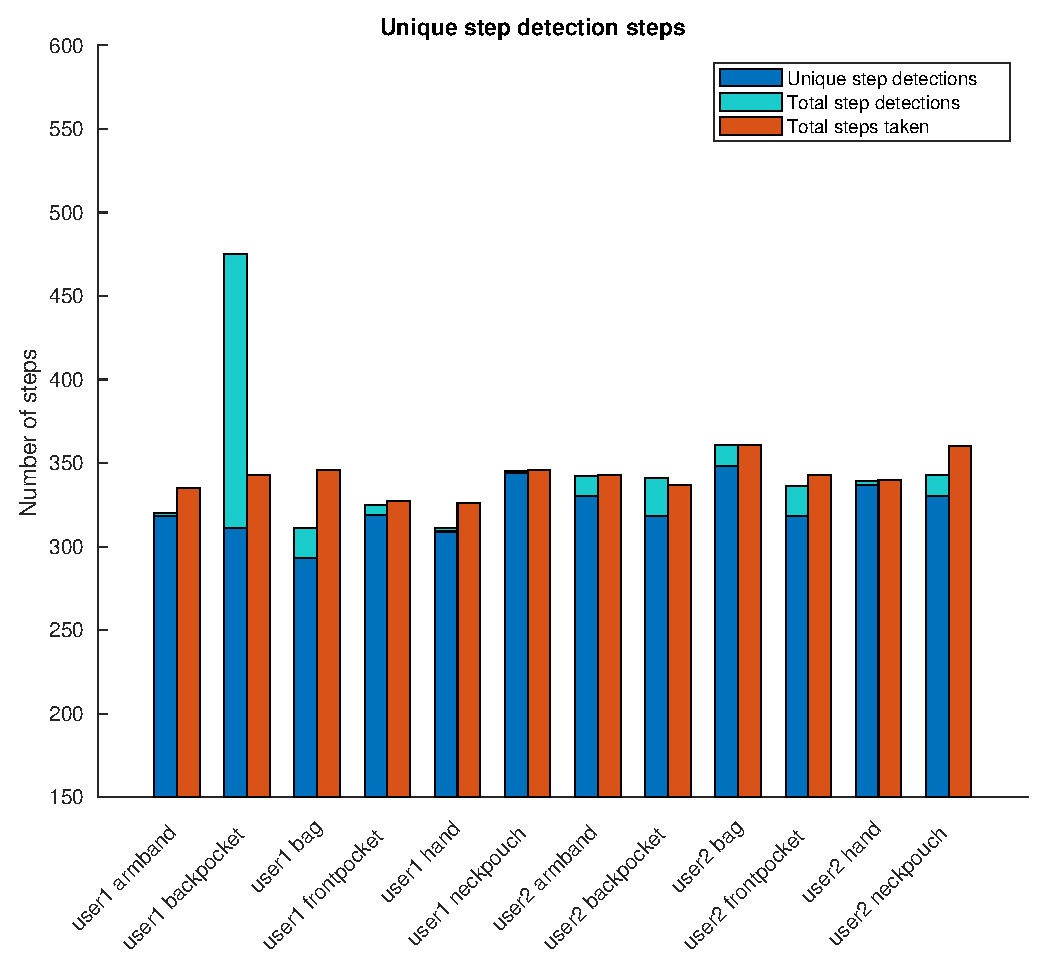
\includegraphics[width=0.7\linewidth]{images/20201127_1626_Unique_step_detection_steps}
	\setlength{\belowcaptionskip}{-10pt}
\caption[False positives and true positives step detection comparison]{Highest unique steps detected using interval method vs total number of steps taken using the step detection method in \cref{sec:meth - step detection}. \citet{Brajdic2013} dataset is used. }
\label{fig:sd_tp_fp_comparison}
\end{figure}

These results show that the number of unique steps is close to the total number of detections, indicating that the step detection method is relatively good at uniquely determining when steps are taken. \par 

From all results in step detection, the in front, with smartphone screen pointing up carrying mode has proven to be the best with low total counting error, small time differences to ground truth steps, and little to no double detections of the same step. This is likely caused by the fact that when held in hand, the smartphone is more or less attached to the user and has little possibility to wiggle in its constraints, in contrast to when the device is placed in pockets. 

\subsection{Step Length Estimation Testing}
\label{sec:results-step_length_estimation}
For step length estimation, the linear relationships between dependent variables and step length, outlined in \cref{sec:rw - step detection}, need to be determined using step detection method in \cref{sec:meth - step detection}. The step detection algorithm cannot guarantee that all steps are counted, potentially affecting the tunable parameter for both methods.  From \cref{sec:rw - step detection} the best performing algorithm for global parameters according to \cite{Vezocnik2019} is reiterated for convenience,

\begin{equation}
	\label{eq:Tian2016_sle2}
	\text{step size} = K_1 h \sqrt{F}.
\end{equation}


where $h$ is the user's height and $F$ is the step frequency. The linear relationship between step length and the dependent variables is defined by $ K_1 $, a tunable parameter. \par 

The best algorithm for individual parameters is 

\begin{equation}
	\text{step size} =K_2 \sqrt[4]{A_{\max }-A_{\min }},
	\label{eq:weinberg_stepsize2}
\end{equation}

where $A_{\max}$ and $A_{\min}$ are the maximum and minimum acceleration within a step interval. The two approaches will be implemented and compared to see if similar results are achieved as within \cite{Vezocnik2019}, and to determine which to use in the indoor localization scheme.

\subsubsection{Online Data}

\citet{Vezocnik2019} have made their accelerometer data available under an open license, consists of smartphone accelerometer data of 15 different people for three walking speeds and in different carrying modes, including in front of the torso and in hand with the screen pointing up. This carrying mode will be used for step length estimation in this section since it performed best in step detection and is used for heading estimation. \par 
Within the dataset, metrics for each test subject are collected, including height, gender, and leg length. The walking speeds were defined qualitative, in that they were either slow, normal, or fast. Each person has two measurements for each walking speed, one for a 15-meter long straight path and another for a 108-meter long straight path. Within \cite{Vezocnik2019}, the smaller distance data set is used to determine parameters for step length estimation methods, while the longer distance data set is used as a performance measure. This same process will be used to determine the performance of step detection and step length estimation. First, the tuneable parameters $ K_1$ and $ K_2$ will be determined using the shorter length walking distances in the opensource data and the step detection method of \cref{sec:meth - step detection}. \par 

\subsubsection{Parameter Estimation}
\label{sec:results-step_length-parameter_estimation}
In \cref{fig:step_length_tian}, the dependent variables of \eqref{eq:Tian2016_sle2} are plotted against average step length. The data from the smaller distances in the \citet{Vezocnik2019} dataset are used. The average step length is calculated by dividing the distance traveled by the number of steps detected. In the figure, each test subject is shown as a different color with the form of the different markers indicating the speed at which that trial was walked at. The positive upward trend indicated in \eqref{eq:Tian2016_sle2} can be observed for all test subjects as walking speed increases. In order to find the universal constant $K_1$ in \eqref{eq:Tian2016_sle2}, a linear least square estimation is performed across all test subject data points. The result is shown by the green striped line in \cref{fig:step_length_tian}, where $ K_1 = 0.3116$. \par 

A similar plot is shown in \cref{fig:step_length_weinberg}, using the same data as in \cref{fig:step_length_tian} but for the  dependent variables \eqref{eq:weinberg_stepsize2}. These are the maximum and minimum acceleration between detected steps. Here to the positive trend indicated by \eqref{eq:weinberg_stepsize2} can be noticed. Since \eqref{eq:weinberg_stepsize2} works best for personalized variable the tunable parameter $ K_2 $ is calculated per test subject, instead of all together as with \eqref{eq:Tian2016_sle2}. This is also done through the linear least square approach.

	\begin{figure}[H]
	\centering
	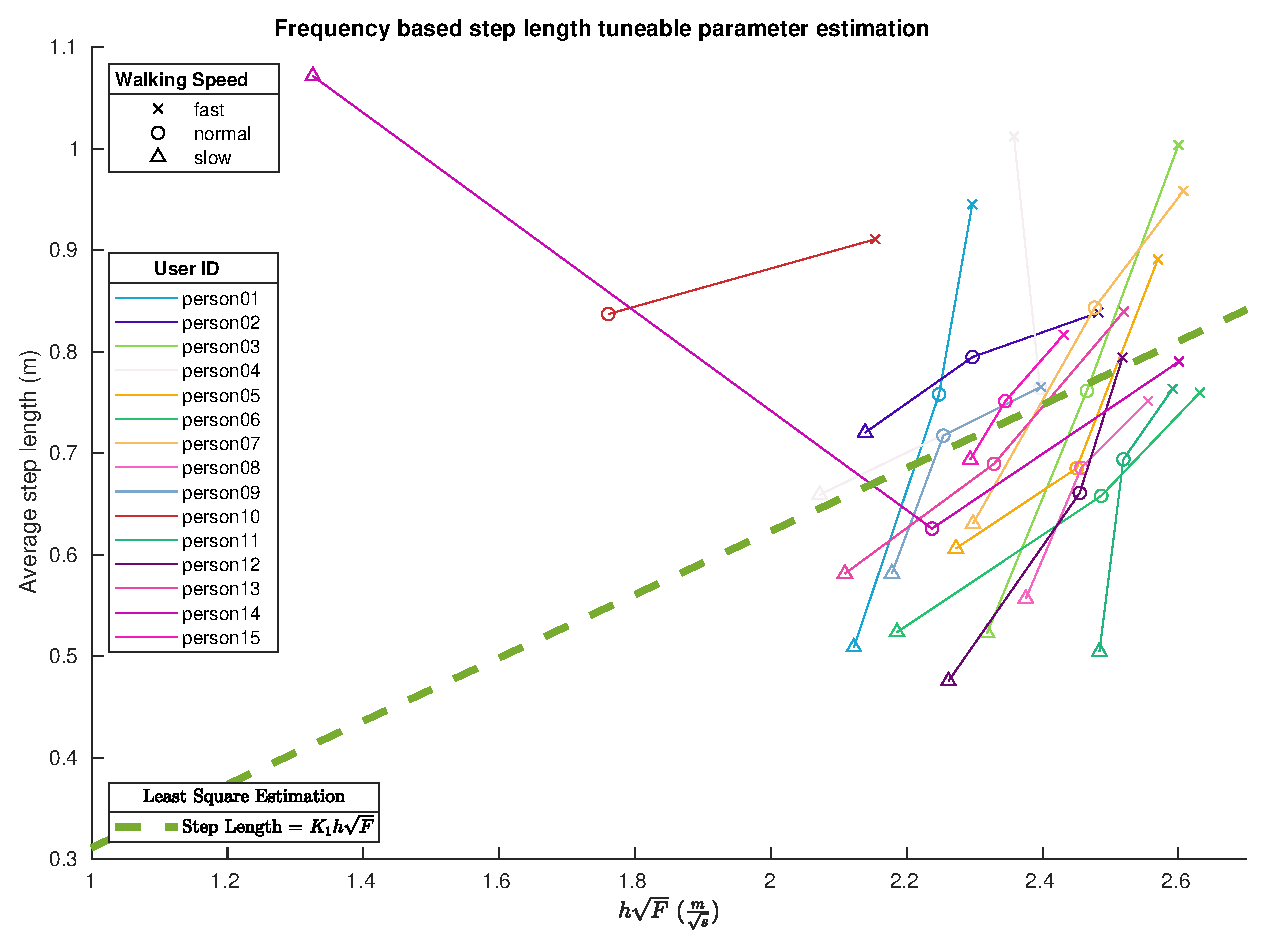
\includegraphics[width=0.8\linewidth]{images/20201128_1304_}
	\setlength{\belowcaptionskip}{-10pt}
	\caption{Dependent variables of \eqref{eq:Tian2016_sle2} plotted against average step length over the smaller distances in the \citet{Vezocnik2019} dataset with step detection from \cref{sec:meth - step detection}. Green striped line represents \eqref{eq:Tian2016_sle2}, where $ K_1 = 0.3116$.  }
	\label{fig:step_length_tian}
	\end{figure}

\begin{figure}[h]
	\centering
	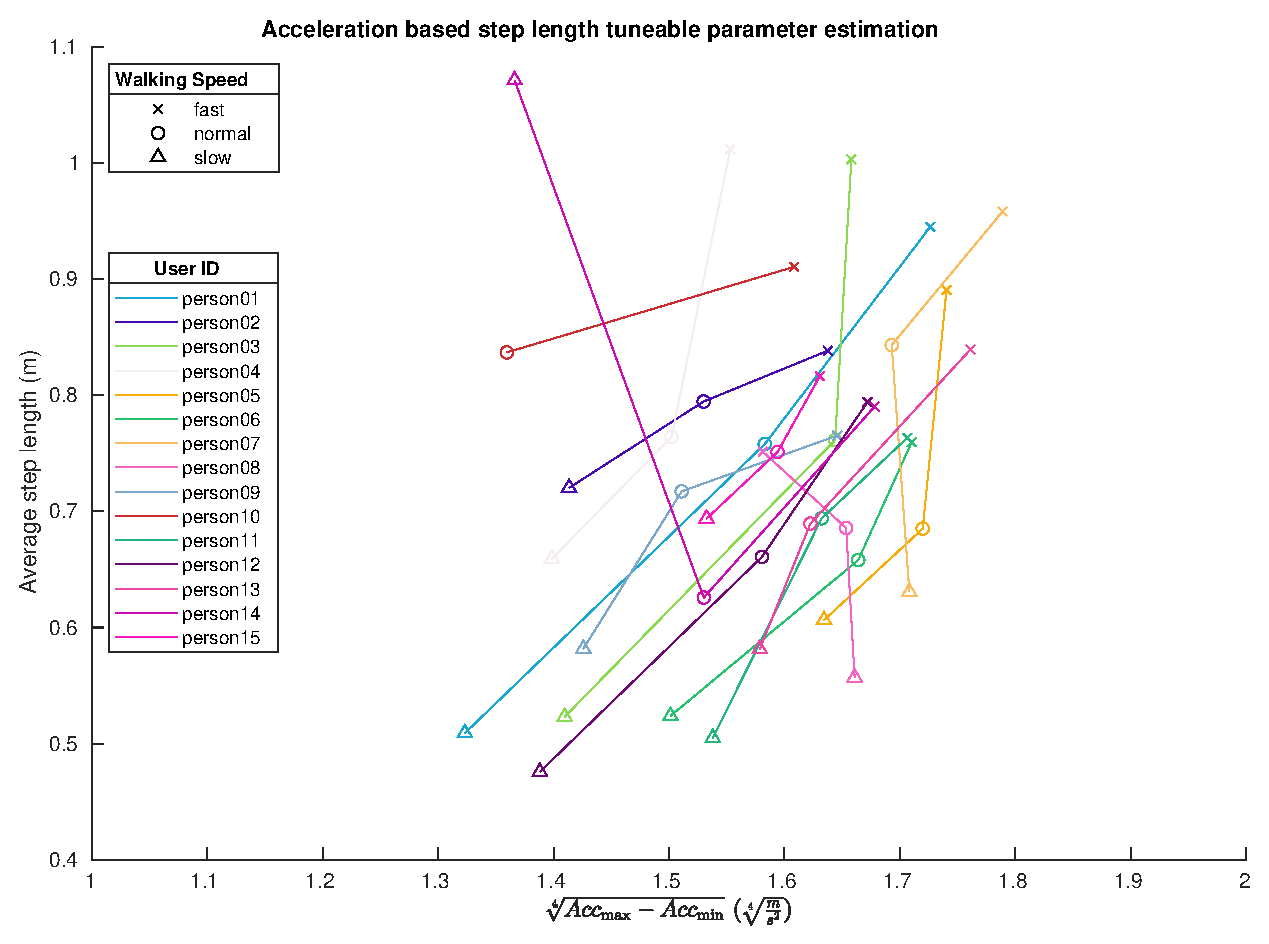
\includegraphics[width=0.8\linewidth]{images/20201128_1317_}
	\setlength{\belowcaptionskip}{-10pt}
	\caption{Dependent variables of \eqref{eq:weinberg_stepsize2} plotted against average step length over the smaller distances in the \citet{Vezocnik2019} dataset. The value of $ K_2 $ is determined per user.}
	\label{fig:step_length_weinberg}
\end{figure}

While most data seems to follow the general linear relationship for both approaches, two samples do not. The two potentially faulty data points are the slow walking sample of both person 10 and 14. For the former, no steps have been detected and are therefore not visible in the plots, while for the latter too few steps have been detected. \par 

For test person 14, 14 steps have been detected for slow walking, which is fewer steps than when the subject was walking fast. This is either a wrong step detection occurring, or the user walks slowly with very large steps. It is difficult to determine why this is occurring. It could be that during this sample, the test subject was holding the phone incorrectly, the person had a very different step strategy when performing at this speed, or the phone was malfunctioning. \par 

This outlier affects the eventual tunable parameter for both step length approaches. Removing it will change the estimate of $K_1$ from 0.3116 to 0.3080. The validation dataset can be used to determine if the difference in the tunable parameter has a significant effect on the total distance traveled. The difference was found to have a negligible effect on the outcome of the method.
%The results are found in  \cref{fig:step_length_estimation_validation}, where the absolute distance error for all walking speeds for all test subjects are shown, indicated by the dataset ID.
%\begin{figure}[H]
%	\centering
%	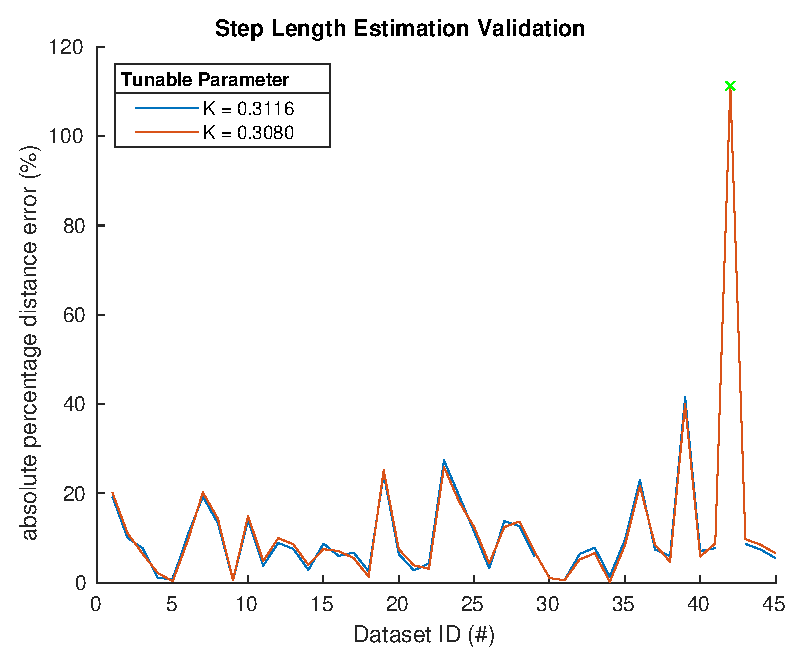
\includegraphics[width=0.65\linewidth]{images/20201028_1344_Step_Length_Estimation_Validation}
%	\setlength{\belowcaptionskip}{-30pt}
%	\caption{Step length estimation using validation dataset}
%	\label{fig:step_length_estimation_validation}
%\end{figure}

\subsubsection{Step Length Method Validation}
\label{sec:results-step_length-validation}
The performance of both step length estimators is evaluated by applying them to the data sets with the long walking distances in the \citet{Vezocnik2019} dataset. In this set, the total distance traveled is recorded by the researchers. The estimated total distance from both \eqref{eq:Tian2016_sle2} and \eqref{eq:weinberg_stepsize2} can be compared with the actual distance walked. The results are shown in  \cref{fig:202011131943_wienberg_vs_tian_vezocnik_data1}. This data surprisingly shows that depending on the test subject one or the other method is better at estimating distance traveled at different walking speeds. This does not coincide with the results of \cite{Vezocnik2019}, where \eqref{eq:weinberg_stepsize2}, which uses personalized parameters for $ K_2 $, performed better than \eqref{eq:Tian2016_sle2}, which uses universal parameters for $ K_1 $. \par 

What is noticeable from the results is that there is an outlier. This is with the slow walking speed of test subject 14, which is also the test subject with which the tunable parameter estimation had an outlier. This further supports that there is something significantly different when this test subject is performing at this walking speed.\par 

 Without the outlier, the mean absolute error for \eqref{eq:Tian2016_sle2} method is 9.7 percent with a standard deviation of 8.0 percent. For the \eqref{eq:weinberg_stepsize2} method the mean is 10.38 percent error with a standard deviation of 7.8 percent error. Both results differ from those cited by \cite{Vezocnik2019}, which indicate a mean of 7 percent with a standard deviation of 5 percent for the former and 3 percent with a 2.5 percent standard deviation for the latter.
 The difference in performance between the literature and the result found here could be caused by the difference in step detection methods, which \cite{Vezocnik2019} does not state explicitly.

\begin{figure}[H]
	\centering
	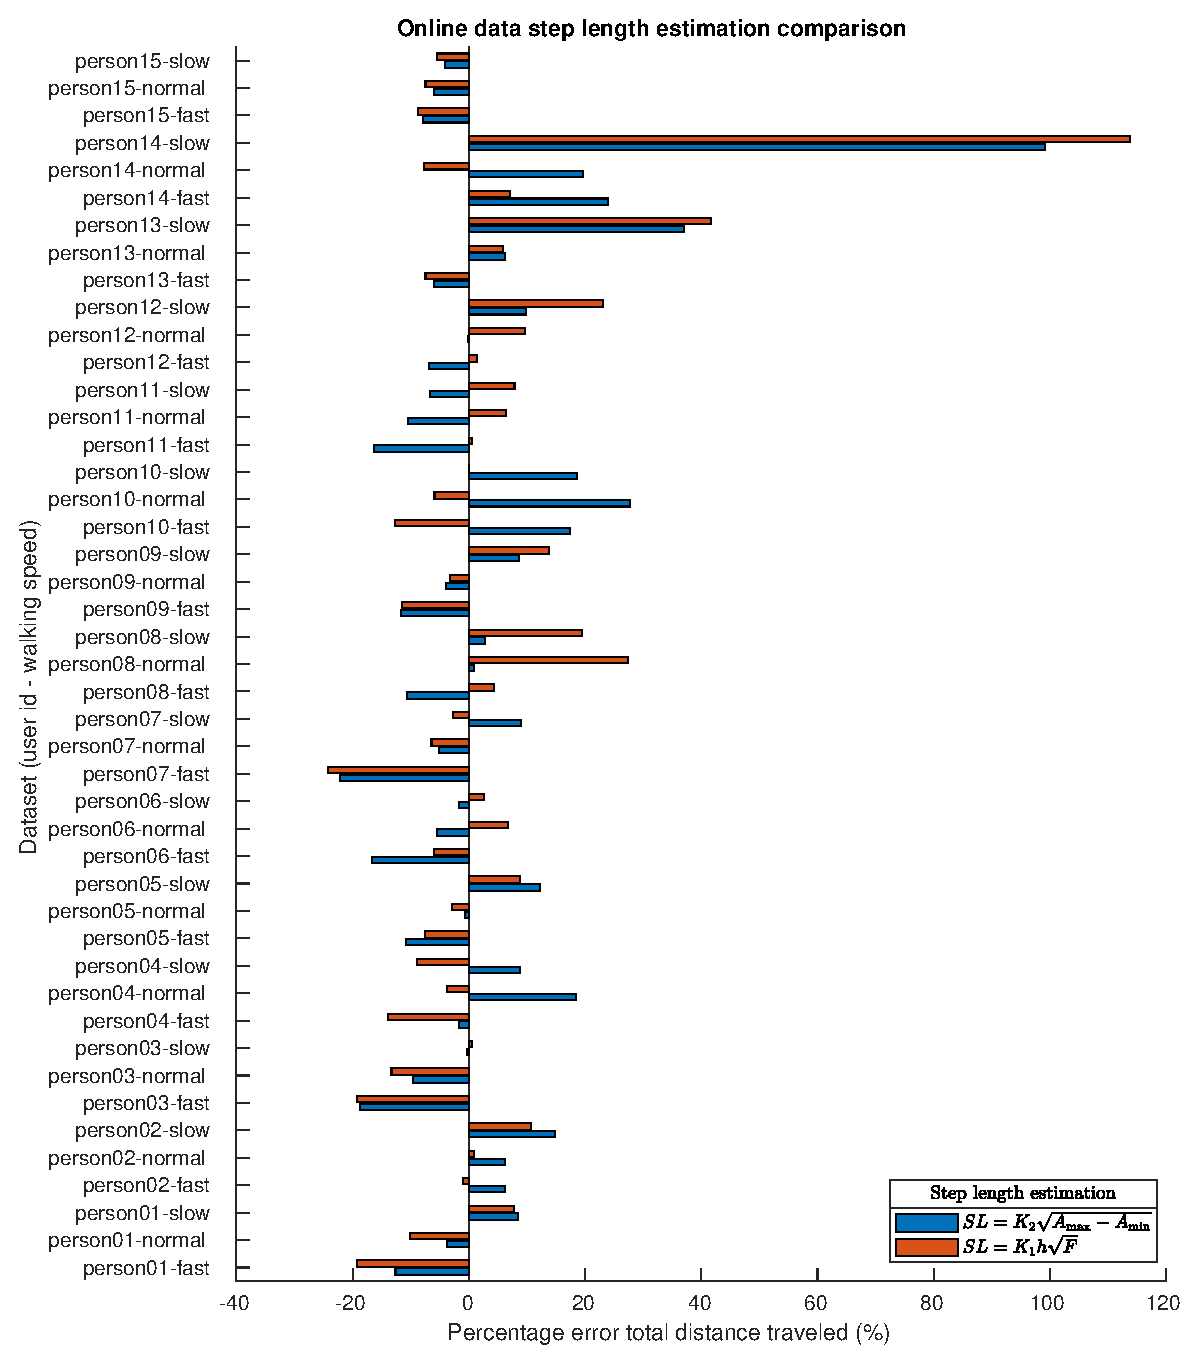
\includegraphics[width=\linewidth]{images/20201128_1403_Online_data_step_length_estimation_comparison}
	\caption{Total distance traveled estimation error from in front, in hand carrying mode from long distance data from \citet{Vezocnik2019} dataset, using \eqref{eq:Tian2016_sle2} and \eqref{eq:weinberg_stepsize2} with step detection from \cref{sec:meth - step detection}. }
	\label{fig:202011131943_wienberg_vs_tian_vezocnik_data1}
\end{figure}
 
Since no conclusive result could be distilled from applying the methods to the opensource data, a small scale experiment was performed outdoors. Within the experiment, the same process as in \cite{Vezocnik2019}, where a small distance data set was collected for parameter $ K_1 $ and $ K_2 $ estimation and a longer data set for performance measurement. Experimental data was collected from the same person and device used in the eventual indoor localization experiment. The smartphone was held in front of the torso and in hand as in \cref{fig:experiment_carrying_position}. \par 

Three trials of 30 meters were walked at different qualitative walking speeds, slow, normal, and fast, while recording accelerometer data. Four longer trials of 300 meters were walked for model validation, also at different walking speeds. All trials were walked with the smartphone in the same carrying mode. \par 

During the smaller walking distances, the number of steps taken was counted manually. For two trials the number of steps detected was exactly the number of steps taken. This was for slow and fast walking where 67 and 50 steps were counted respectively.  For the other trial, the detection of \cref{sec:meth - step detection} was off 2 steps, with 57 steps being taken and 55 being recorded. With these small step counting errors indicating that step detection is working properly, errors in step length estimation are likely not caused by wrongful step detection.  \par 

The different step length estimation methods were applied to the experimental accelerometer data. The same parameter $ K_1 $ determined for the online dataset was used for model validation with the experimental data. The $ K_2 $ parameter was estimated on the smaller distance data. The results are shown in \cref{fig:step_length_personal_testing}. The results suggest that for slow to normal walking step detection using \eqref{eq:Tian2016_sle2} works best, with a chance of underestimating the distance traveled. For normal to fast walking, using \eqref{eq:weinberg_stepsize2} for step detection works better, with a chance of overestimating the distance traveled. By assuming that walking indoor is generally more in the normal to slow speed range, the choice was made to use the \eqref{eq:Tian2016_sle2} method for step length estimation in the indoor localization system.
\begin{figure}[H]
	\centering
	\includegraphics[width=0.7\textwidth]{images/20201128_1430_original_data_step_length_estimation_comparison}
		\setlength{\belowcaptionskip}{-15pt}
	\caption{Step length estimation method comparison using experimental accelerometer data recording while walking and step detection from \cref{sec:meth - step detection}. }
	\label{fig:step_length_personal_testing}
\end{figure}

For both the opensource data and the experimental data, the accelerometer-based method in \eqref{eq:weinberg_stepsize2} does not necessarily work better than the frequency-based method in \eqref{eq:Tian2016_sle2}, in contrast to what \citet{Vezocnik2019} indicated. For future work, it may be worthwhile to test the other algorithms outlined te{Vezocnik2019} to see if there are any other differences between the outcomes. \par 

Another observation that can be made from the above results is that the linear relationships of both \eqref{eq:Tian2016_sle2} and \eqref{eq:weinberg_stepsize2} are ill-fitted to the data that is used for parameter estimation in \cref{sec:results-step_length-parameter_estimation}. The models are theoretically sound, in that they intersect with the origin. For the models, this corresponds to zero frequency having a step length zero, and no difference in acceleration difference within a step interval having a step length of zero. This is what is expected for these values. From the figures for parameter estimation of both models, this perspective is not shared. While there does seem to be a general positive linear trend, the slopes are much steeper than the origin intersecting linear model. Fitting a linear model using this observation would require adding an offset to the different models, of the form

\begin{align}
	\text{step size} &= K_1 h \sqrt{F} + c_1. \\
	\text{step size} &= K_2 \sqrt[4]{A_{\max }-A_{\min }} + c_2,
\end{align}

where $ c $ is the offset applied to the different models. Applying these offsets will make the models work only within an interval of frequencies and acceleration differences since step length cannot be negative. This will have to be researched further in future work.


\subsection{Indoor Orientation Estimation}
\label{sec-results-Indoor orientation_estimation}
The step heading component of the Step and Heading System is tested using the data from the indoor experiment. This was required since it was designed to handle magnetic disturbance found within the built environment.\par 
Determining the performance of orientation estimation during the indoor experiments is difficult since no ground truth was available for comparison. A sanity check that can be performed is comparing the orientation estimations of the EKF in \cref{sec:meth-indoor_heading_estimation} with the orientation estimations calculated by the Android operating system. The results will not be able to indicate performance with respect to the actual orientation, but could potentially highlight any very diverging behavior. \par 

In order to calculate an orientation difference, a difference quaternion ($	\Delta q_t$) can be used, defined as \cite{Kok2017}

\begin{equation}
	\Delta q_t = \hat{q}_{t}^{nb} \odot \left( \hat{q}_{comp,t}^{nb}  \right)^c,
\end{equation} 

where $\hat{q}_{comp,t}^{nb}$ is the unit quaternion that $ \hat{q}_{t}^{nb} $ is compared with.  In order to compare the orientation estimates of the android system and the EKF from \cref{algo:indoor_EKF}, the difference in angle between the first quaternion estimate and the following quaternions estimate is calculated for both orientation estimates, since both do not necessarily share the same reference frame. This is done to calculate the relative orientation estimate to the initial orientation. It is also this relative orientation that is used by the \ac{SHS}.\par 

Since both relative orientation estimates start at the same initial quaternion, namely the zero quaternion. the two estimates can now be compared. Applying the difference quaternion calculation between the two relative orientation estimates, the difference quaternions over the whole orientation estimate are determined.  \par 

Once calculated, the difference quaternions can be converted into Euler angles for more intuitive interpretation. The mean difference in the yaw component for each trial is shown in  \cref{fig:yaw_difference_between_android_and_ekf_1}. From the results, the difference between orientation estimations seems larger for trials 5 and 6, requiring further investigation.

\begin{figure}[H]
	\centering
	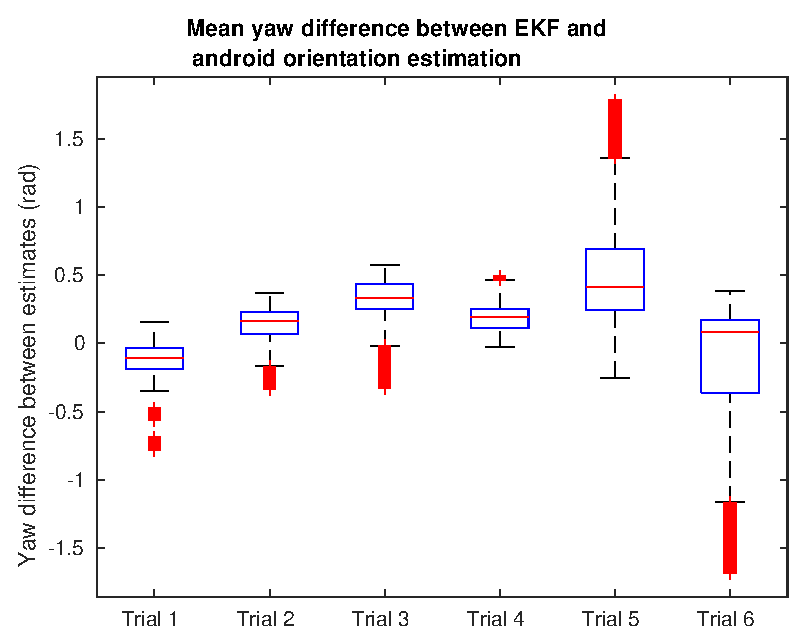
\includegraphics[width=0.7\linewidth]{images/20201201_1212_Mean_yaw_difference_between_EKF_android_1}
	\setlength{\belowcaptionskip}{-10pt}
	\caption{Yaw difference between EKF estimate in \cref{algo:indoor_EKF} and android orientation estimates. Trial 5 and 6 show a much larger spread in yaw difference with the orientation estimate of the android phone. The red markers represent outliers in the box and whisker plot implementation.}
	\label{fig:yaw_difference_between_android_and_ekf_1}
\end{figure}

The yaw traces of the android system and EKF for trial 5 and 6 can be found in \cref{fig:trial5_yawdifferencebetweenmethods} and \cref{fig:trial6_yawdifferencebetweenmethods}, respectively. At the start of the orientation estimation, a large jump between 1.4 and 1.8 rad by the EKF can be noticed for both trials, which slowly converges back to the orientation estimate of the android operating system. This is not present in trials 1 to 4. It is not clear what is causing this spike, but it is evident that this can affect the SHS output, and potentially the position estimate of the Particle Filter. One hypothesis is that the initial orientation state is far off reality. The large initial covariance at this time point allows the EKF in \cref{algo:indoor_EKF} to make a large estimate jump when a magnetometer measurement update occurs. Using a prior estimating technique such as the TRIAD algorithm \cite{Kok2017} could be used to mitigate this in the future. \par 

Although not ideal, it is still possible that the Particle Filter can handle this jump, since the Particle Filter uses the \textit{change} in step heading between steps to alter the heading of the particles, not the heading itself. From the figures, a qualitative observation can be made that the general trend of the yaw estimate does seem to coincide with that of the Android system, albeit with an offset caused by the yaw jump at the start. If the yaw jump occurs before the first step is set, then only the slight drift back will affect the \ac{SHS} output. \par 

In the case that these trials are unable to complete the Particle Filter runs correctly, the orientation estimate of the phone can be used to determine if it is caused by the orientation estimate of \cref{sec:meth-indoor_heading_estimation} or not.
\newpage
\newgeometry{left=3cm,bottom=0.1cm}
\begin{figure}[H]
	\centering
	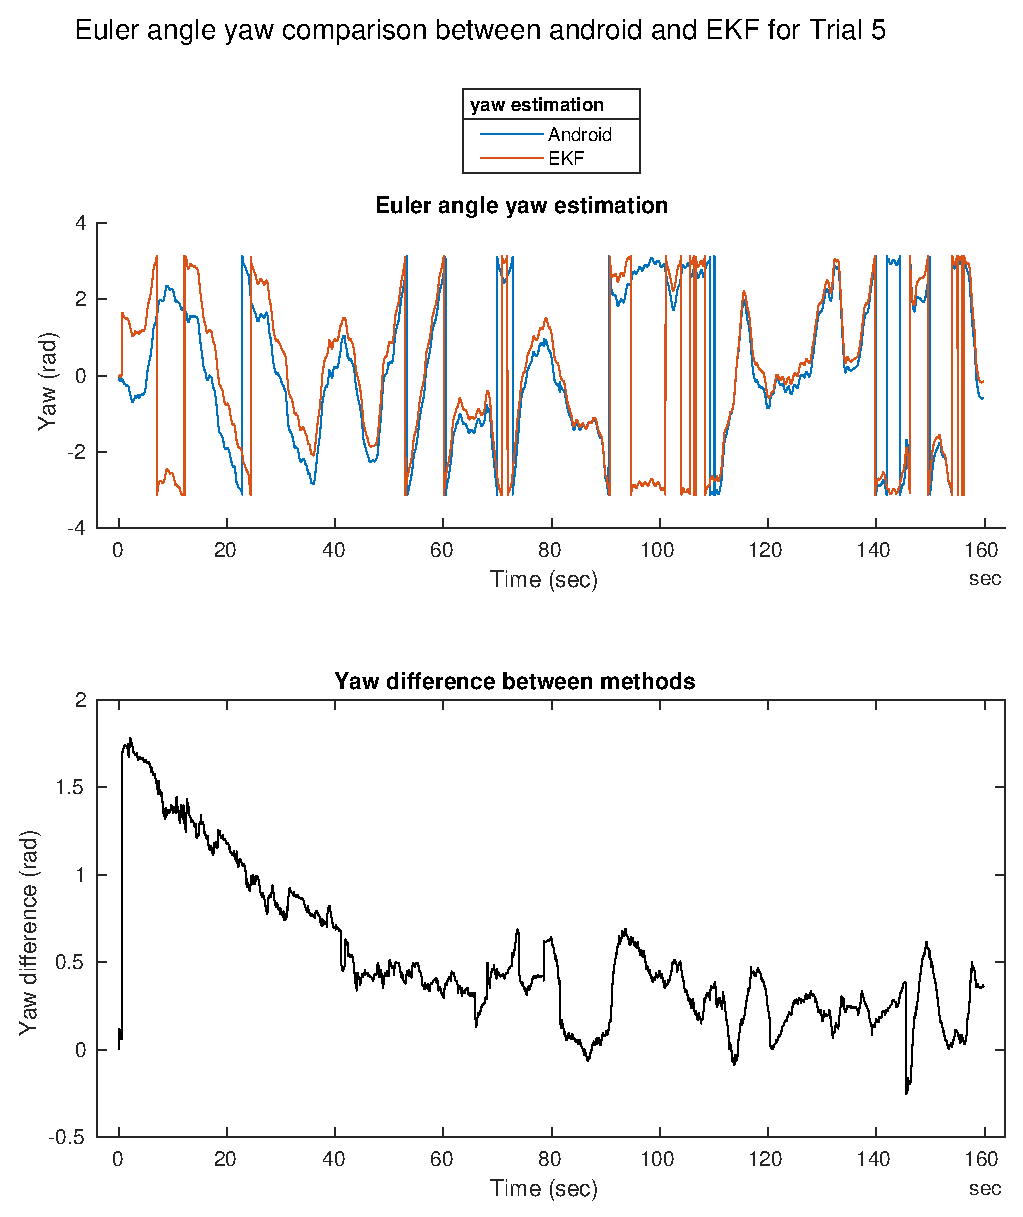
\includegraphics[width=0.6\linewidth]{images/20201201_1218_Yaw_difference_between_methods}
	\setlength{\belowcaptionskip}{-20pt}
	\caption{ Yaw comparison between Android and EKF from \cref{sec:meth-indoor_heading_estimation} of trial 5.}
	\label{fig:trial5_yawdifferencebetweenmethods}
\end{figure}
\begin{figure}[H]
	\centering
	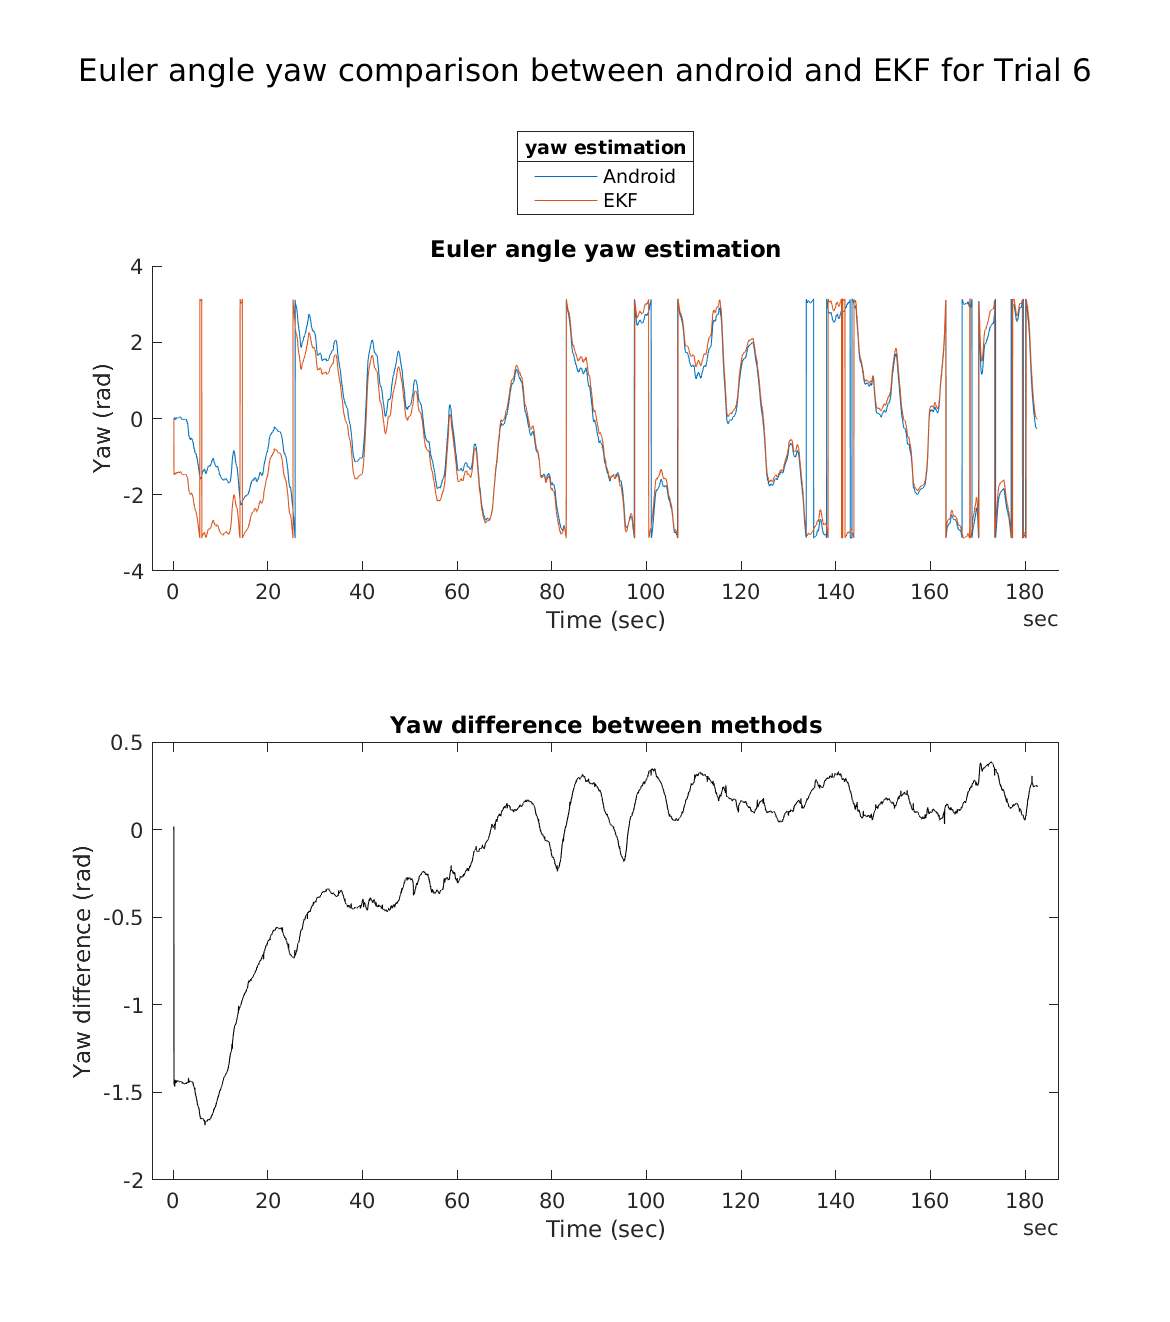
\includegraphics[width=0.7\linewidth]{images/20201201_1219_Yaw_difference_between_methods}
	\setlength{\abovecaptionskip}{-20pt}
	\setlength{\belowcaptionskip}{-20pt}
	\caption{Yaw comparison between Android and EKF from \cref{sec:meth-indoor_heading_estimation} of trial 6.}
	\label{fig:trial6_yawdifferencebetweenmethods}
\end{figure}
\restoregeometry
\newpage
\subsection{Step and Heading System Trajectories}
\label{sec:results-SHS_trajectories}
The \acl{SHS} alone is not a viable position estimate. It generates a relative trajectory and has no way to align itself with the indoor environment. The particle filter translates the relative trajectory to an absolute one, respecting the spatial constraints.\par 

While no reasonable quantitative comparison can be done between \ac{SHS} output and camera position estimate, a qualitative comparison can. The SHS trajectory generated from the smartphone IMU during indoor testing can be heuristically rotating to fit the general video estimate, producing \cref{fig:trial1_shs_gt_comparison} and \cref{fig:trial6_shs_gt_comparison}, for trial 1 and 6 respectively .\par 

Some observations can be made from this qualitative approach. First, for trial 1, the general trend along the x and y-axis of the SHS output is comparable to that of the video estimate, as can be seen in \cref{fig:trial1_comparison}. The position of the SHS trajectory of trial 1, as seen in \cref{fig:trial1_on_map}, is also relatively close, although it naturally does not conform with the spatial constraints. \par 
For trial 6 in \cref{fig:trial6_shs_gt_comparison}, the trend of the SHS trajectory shows similar changes in position over time when compared to the video estimate, but with more drift on the y axis. The position of the SHS trajectory in the x-axis follows the video estimate relatively close. The general trend on the y axis also is similar to that of the video position estimate, but the distance error along the axis is over 5 meters most of the time. \par 

This qualitative comparison highlights that the quality between SHS output can vary, where better quality refers to the ability to follow the video estimate better when rotated correctly. Variables that can influence this could be the route walked, which may pass different magnetic disturbances, calibration error, and incorrectly detected steps.

\begin{figure}[H]
	\centering
	\begin{subfigure}[t]{.45\textwidth}
		\centering
		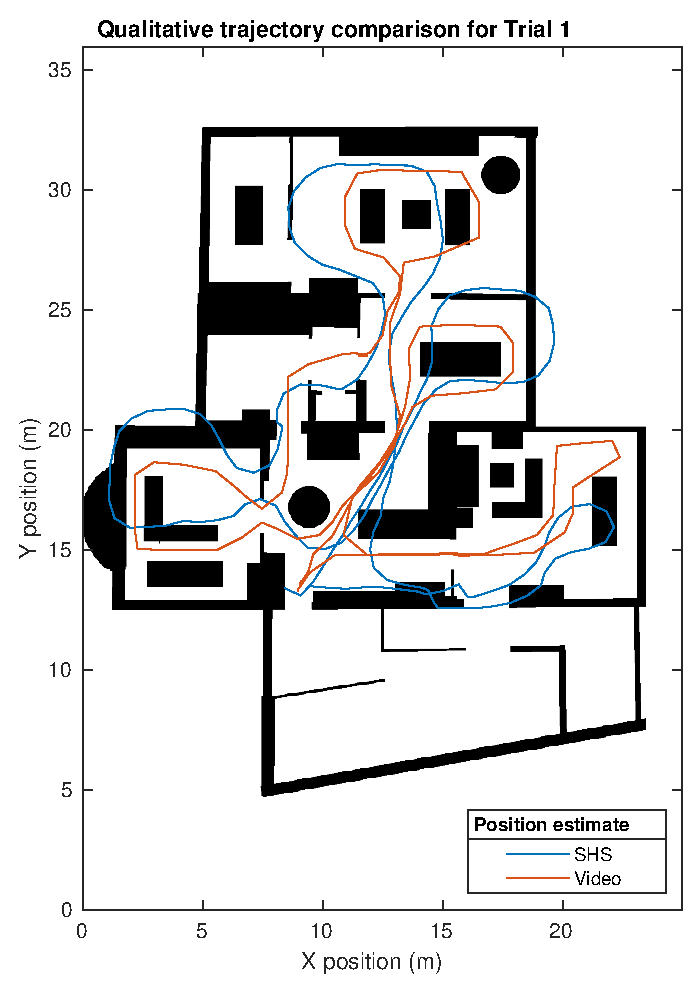
\includegraphics[width=0.85\linewidth]{images/20201201_2209_Qualitative_trajectory_comparison_for_Trial_1_1}
		\caption{trajectory comparison}
		\label{fig:trial1_on_map}
	\end{subfigure}
	\begin{subfigure}[t]{.45\textwidth}
		\centering
		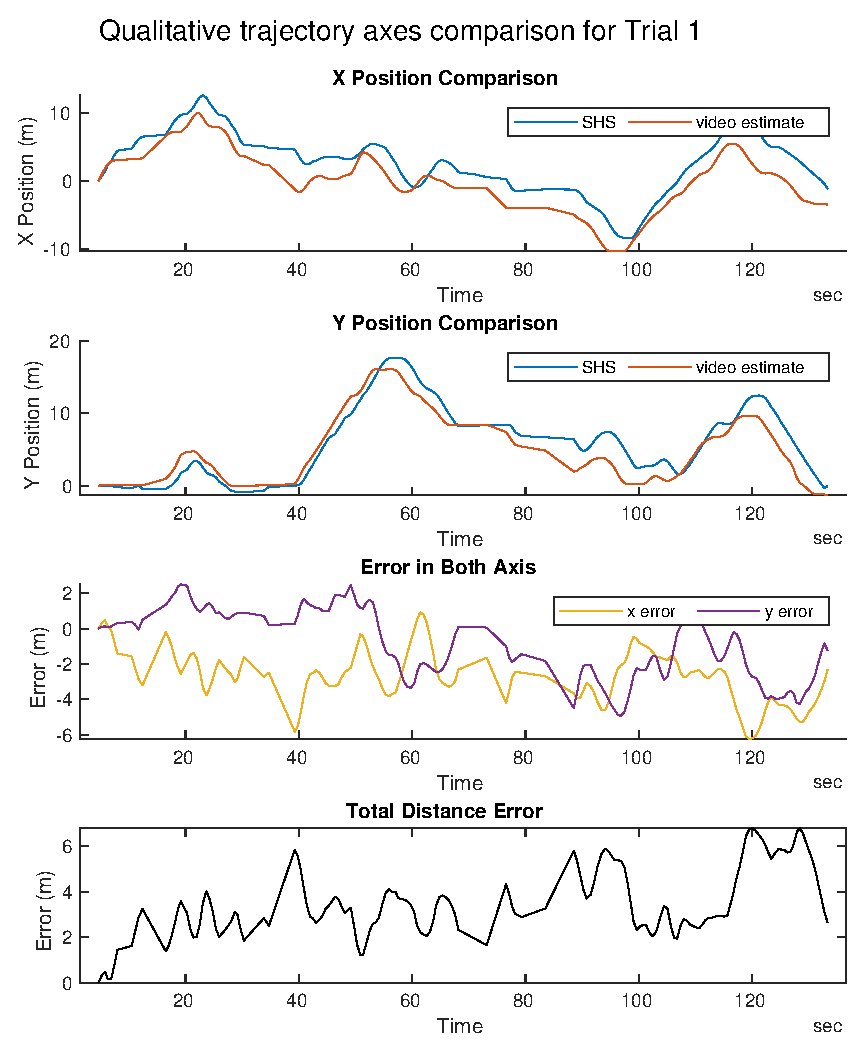
\includegraphics[width=\linewidth]{images/20201202_0913_Qualitative_trajectory_axes_comparison_for_Trial_1_1}
		\caption{axis comparison}
		\label{fig:trial1_comparison}
	\end{subfigure}
\setlength{\belowcaptionskip}{-10pt}
	\caption{Qualitative step and heading system comparison of trial 1 with ground truth}
	\label{fig:trial1_shs_gt_comparison}
\end{figure}

\begin{figure}[H]
	\centering
	\begin{subfigure}[t]{.45\textwidth}
		\centering
		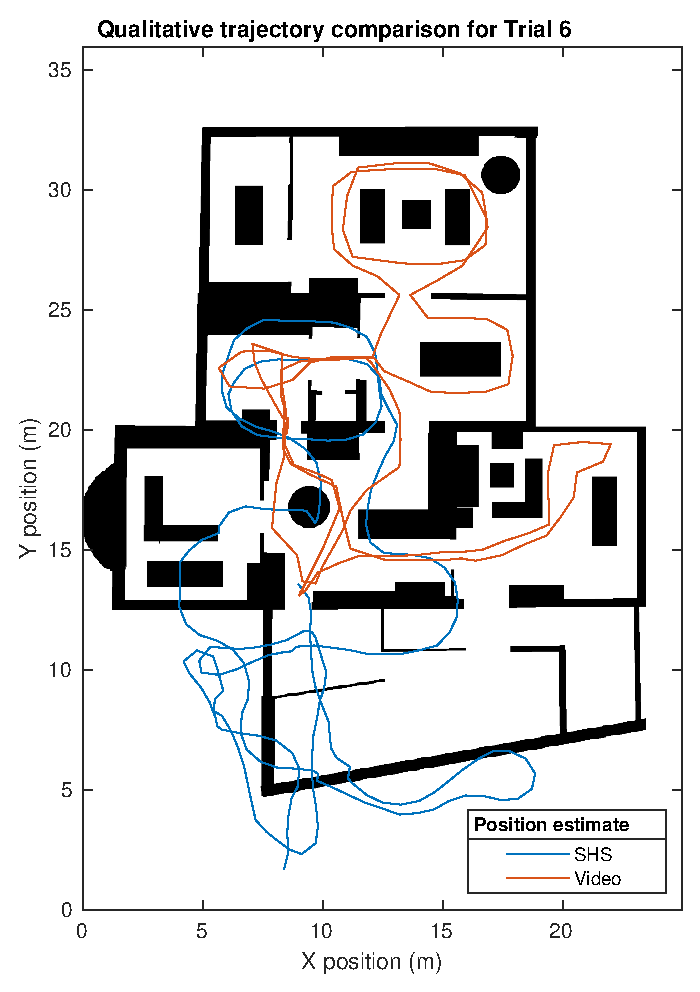
\includegraphics[width=0.85\linewidth]{images/20201201_2220_Qualitative_trajectory_comparison_for_Trial_6_1}
		\caption{trajectory comparison}
		\label{fig:trial6_on_map}
	\end{subfigure}
	\begin{subfigure}[t]{.45\textwidth}
		\centering
		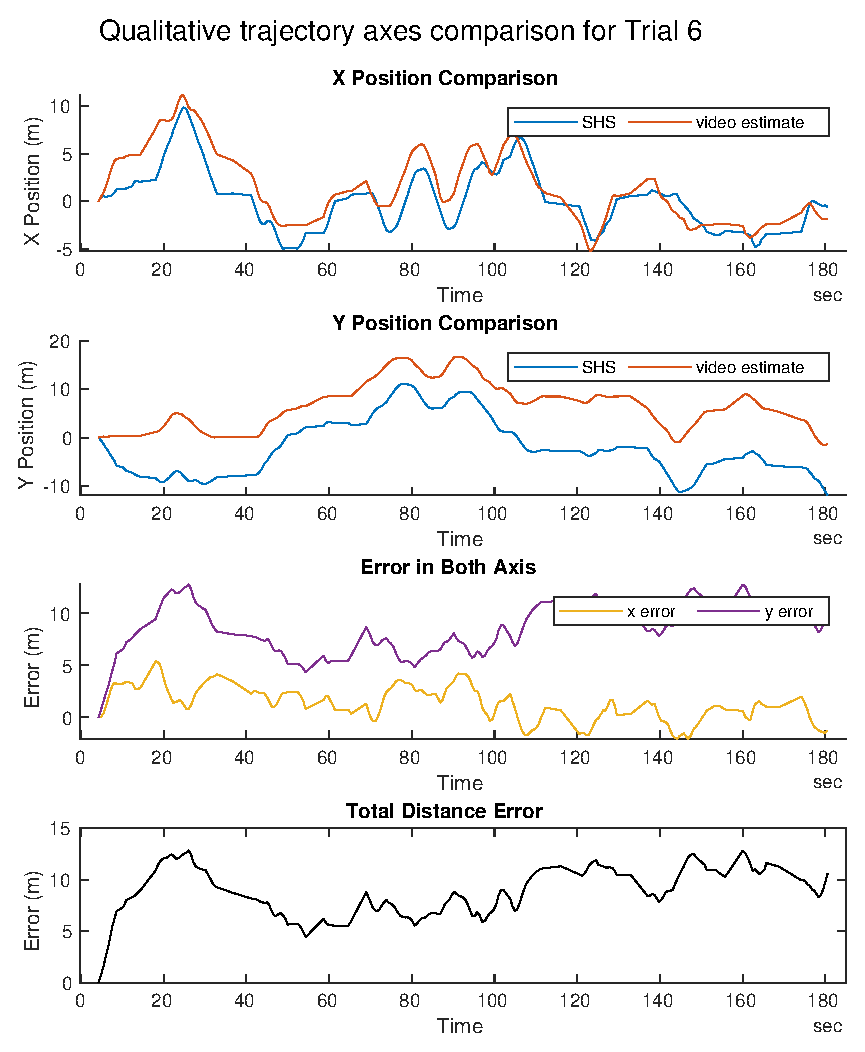
\includegraphics[width=\linewidth]{images/20201201_2253_Qualitative_trajectory_axes_comparison_for_Trial_6_1}
		\caption{Axis comparison between video estimate and heuristically rotated SHS trajectory.}
		\label{fig:trial6_comparison}
	\end{subfigure}
\setlength{\belowcaptionskip}{-20pt}
	\caption{Qualitative step and heading system comparison of trial 6 with ground truth}
	\label{fig:trial6_shs_gt_comparison}
\end{figure}

\section[SHS-PF Testing]{Step and Heading System Particle Filter Testing}
\label{sec:results-SHSPF}
Through the indoor experiment outlined in \cref{sec:results-experimental setup}, the complete indoor localization system could be tested, from input sensor measurements and map information to position estimate. The IMU data is passed through the \ac{SHS} subsystem of \cref{sec:method-SHS} to produce \ac{SHS} information, consisting of step heading and step length each time a step is detected. The smartwatch IMU data is passed through the activity recognition method in \cref{sec:method-AR} to detect door interaction. Combining the \ac{SHS} data and door interaction detection with the floor map generated in \cref{sec:method-particle_filter}, the Particle Filter propagates position estimates through the indoor environment, while taking spatial context into account. The resulting trajectories from the particles at the last time step of the SHS data are averaged to produce the indoor position estimate over the experiment, as explained in \cref{sec:method-pf_location_estimate}. The whole system combined will be referred to as the Step and Heading Particle Filter (SHS-PF).  \par 

By using the video recordings made during the different trials, a rough position estimate was created. This rough estimate can be used for comparison with the position estimate of the \ac{SHS} Particle Filter, in order to get an indication of the estimating performance. This can be done by calculating the root-mean-square error between the two position estimates as

\begin{equation}
	\displaystyle \operatorname {RMSE} ={\sqrt {\frac {\sum _{n=1}^{N}({\hat {y}}_{n}-y_{n})^{2}}{N}}},
	\label{eq:RMSE}
\end{equation}

where $N$ is the total number of steps detected by the SHS, $\hat{y_n}$ the postion estimate at step $n$ of the SHS-PF and $y_n$ the video trajectory position at the time of the step $n$. \par 

In this section, reference will be made to "Particle Filter runs". A run consists of feeding the Particle Filter the input data multiple times. This is done to get an indication of reproducibility, since the resampling step in the Particle Filter samples from a particle distribution, which is a stochastic process, not necessarily generating the same results each time.\par 
A run is considered completed if there are still particles present at the last time step of the SHS data. The inability to complete a run indicates that the SHS and door interaction inputs are causing all particles to run into spatial constraints at some point and in the process eliminating themselves. This leaves no particle over for the Particle Filter to propagate, hence no further position estimate to produce.

\subsection{SHS-PF without Door Interaction Measurement Update}
\label{sec:SHS-PF_without_door_interaction}
In order to compare the effect that activity recognition has on the performance of the SHS-PF, scenarios must be performed in which they are and are not available. Since different information is available in both cases, it is likely that different model parameters will be needed for the SHS-PF to function properly.\par 

First, the scenario in which door interaction is not available will be handled, hence no Particle Filter door interaction measurement updates will occur. The spatial constraint measurement updates will still occur.

\subsubsection{Determining Particle Filter Time Update Standard Deviations}

The Particle Filter time update presented in \cref{sec:meth-pf-SHS_time_update} uses predefined standard deviations for the noise realizations on step heading and step length. These values are found iteratively by trying different combinations of standard deviations for both variables for all the different experimental trials. Step heading standard deviation is tested between a range of 0.1 to 0.2 rad. Step length standard deviation is tested between a range of 0.1 to 0.2 meters. These intervals were determined empirically. For each combination of parameters, 5 runs are performed, with 2000 particles each.\par 

The parameter sweep of trial 3 can be found in \cref{fig:rmsebetweenvideotrajectoryandshs-pffortrialnodetections31}. The sweeps of other trials can be found in \cref{sec:app-shs_pf_noise_realization_no_detection}. The number at the top of each bar chart indicates how many Particle Filter runs were able to reach the end of the SHS data set with particles still available. This is also shown by the number of bars within each box. The height of the bars indicates the RMSE between the position estimate of the SHS-PF and the video estimate. Higher values indicate trajectories that diverge more from the video position estimate.\par 

\begin{figure}[H]
	\centering
	\includegraphics[width=0.8\linewidth]{"images/20201202_1344_orientation_std:_0_2_rad"}
	\setlength{\belowcaptionskip}{-15pt}
	\caption{Parameter sweep of different standard deviation values for step heading and step length in Particle Filter time update for trial 3 without door detections. The number at the top of each bar graph indicates how many Particle Filter runs were completed, and the bars show the RMSE value for each completed run between the SHS-PF estimate and the video position estimate. }
	\label{fig:rmsebetweenvideotrajectoryandshs-pffortrialnodetections31}
\end{figure}

\subsection{SHS-PF without Door Interaction Performance}

For each trial, the combination of standard deviations was taken where all runs were completed with the lowest RMSE, the result of which can be found in \cref{fig:placeholder}

The results in \cref{fig:placeholder} show that when door interactions are not used trials 3 to 6 have large RMSE values in addition to a wide range. These high values and large spread indicates that the position estimate are different each run and do not coincide with the video position estimate. Trials 1 and 2 have lower RMSE values and the spread is much smaller, with the latter indicating similar estimates between runs, and the former indicating varying degrees of similarity with the video position estimate.\par 

The RMSE value between trials 1 and 2 can be explained by looking at the trajectory that the system generates. The particles for trials 1 and 2 both diverge from the trajectory derived from video analysis at some point. This can be seen for trial 1 in  \cref{fig:shspf_trial1_shs_gt_comparison}, where the particle filter position estimate does not go around the structure circled in green, while the video trajectory does. \cref{fig:shspf_trial2_shs_gt_comparison} shows the position estimate of Trial 2, where the Particle Filter seems to walk too far, through the opening indicated by the green circle and is unable to make the correct turn. \par 

The overall results show that, up to a certain extent, SHS input can be enough for the SHS-PF to estimate a position estimate consistently. It is however possible for the estimate to diverge from the actual pedestrian position.

One hypothesis why one SHS trajectory is better than others relates to \cref{sec:results-SHS_trajectories}, where the qualitative comparison between SHS trajectory and video position. For both trials 1 and 2, the two were able of generating consistent, albeit diverging, estimates had trajectories that followed the video estimate better than trials 3 to 6. Gaining additional insight into a qualitative measure that can represent could present criteria that a SHS trajectory should meet to generate a consistent estimate in this setting. 

\begin{figure}[H]
	\centering
	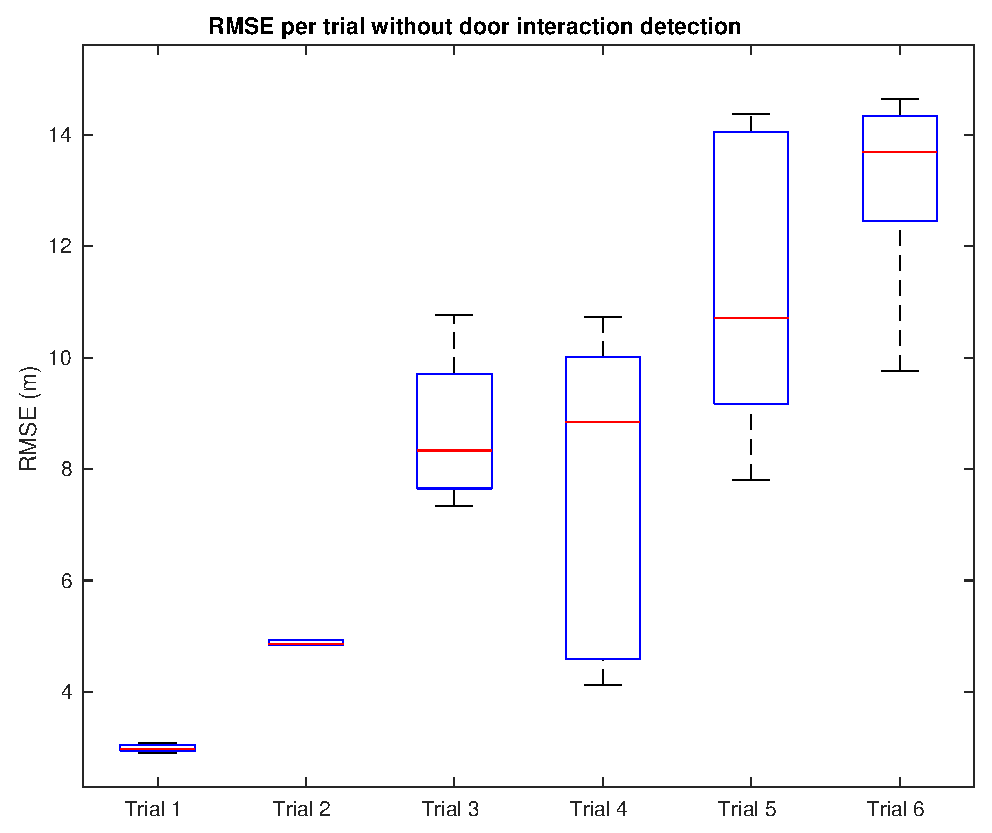
\includegraphics[width=0.7\linewidth]{images/20201202_2216_last_image_for_thesis_1}
	\caption{Root-mean-square error between Particle Filter position estimate and video position estimate.No door interactions were used for Particle Filter measurement updates.}
	\label{fig:placeholder}
\end{figure}



\begin{figure}[H]
	\centering
	\begin{subfigure}[t]{.45\textwidth}
		\centering
		\begin{tikzpicture}
			\node[anchor=south west,inner sep=0] (image) at (0,0) {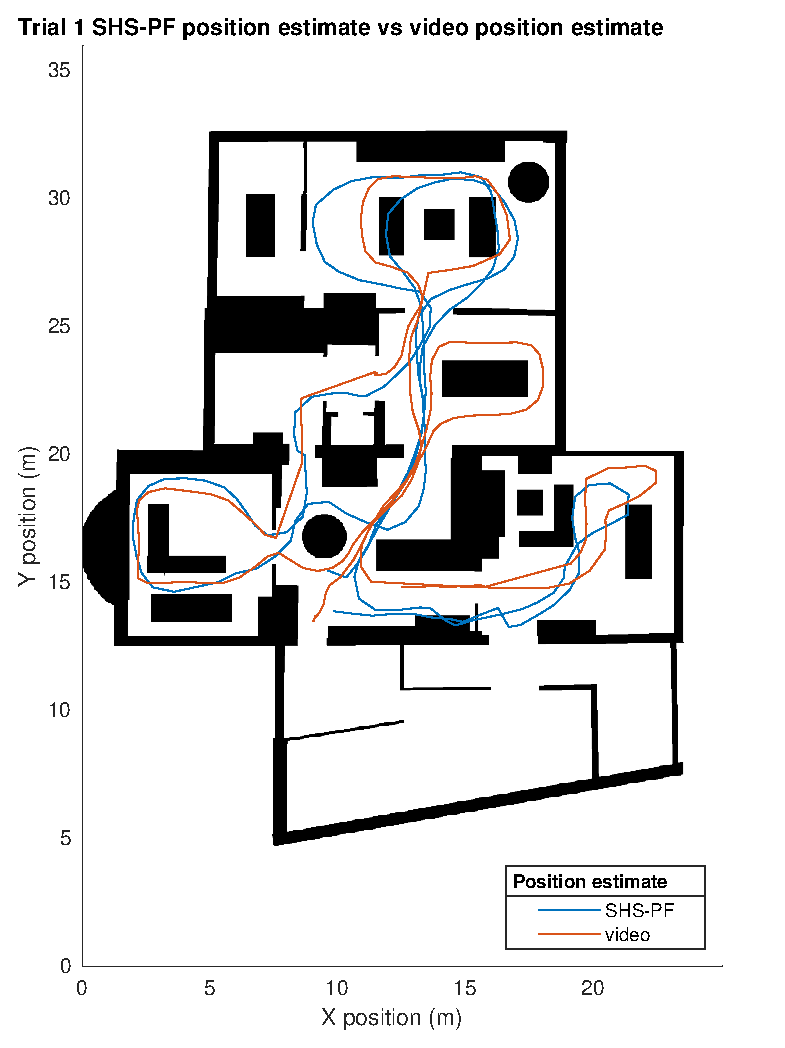
\includegraphics[width=0.91\textwidth]{images/20201129_1907_trial_1_map_1}};
			\begin{scope}[x={(image.south east)},y={(image.north west)}]
				\draw[green,ultra thick,rounded corners] (0.557,0.625) rectangle (0.687,0.66);
			\end{scope}
		\end{tikzpicture}		
		\caption{Position estimate trajectory comparison. }
		\label{fig:shspf_trial1_on_map}
	\end{subfigure}
	\begin{subfigure}[t]{.45\textwidth}
		\centering
		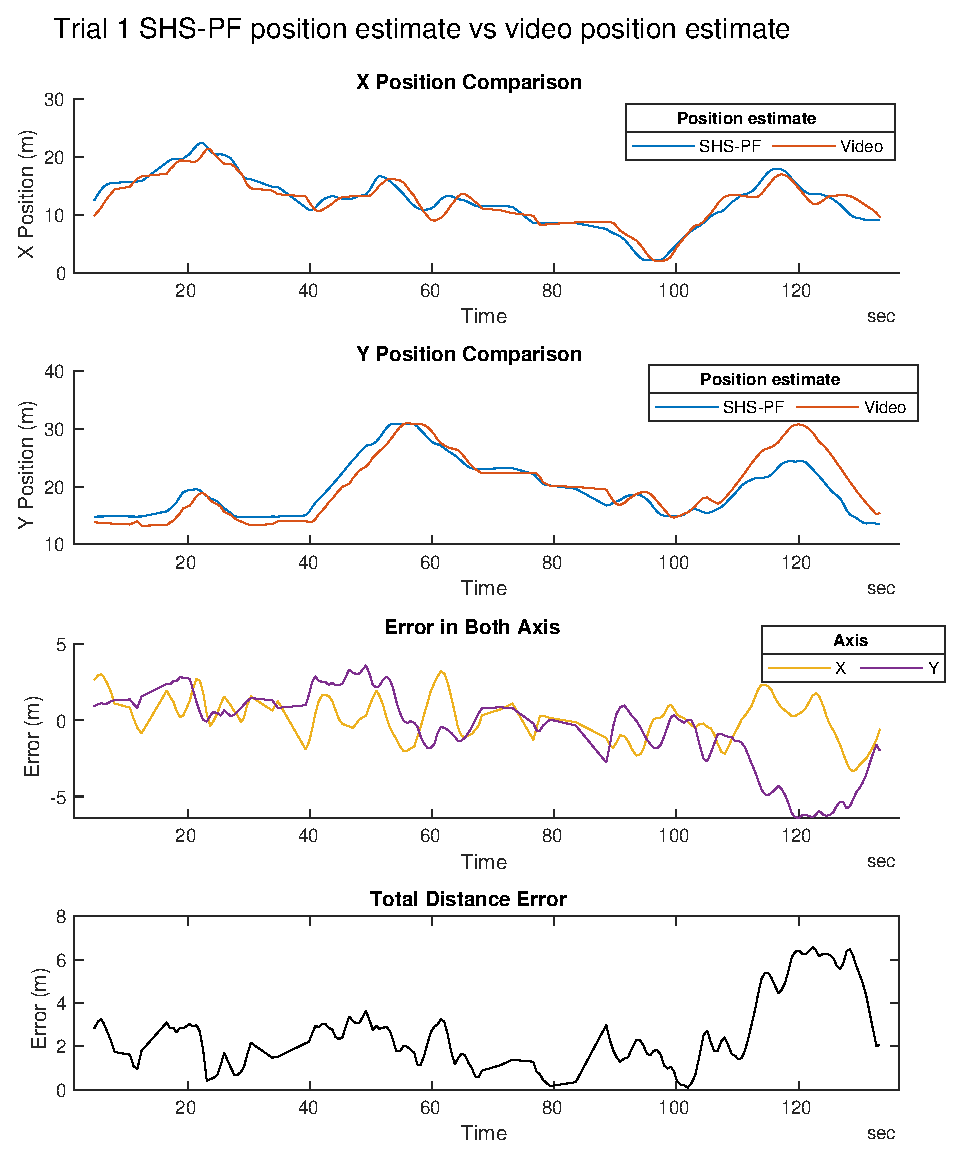
\includegraphics[width=\linewidth]{images/20201129_1946_trial_1_traj_1}
		\caption{Position estimate axis comparison.}
		\label{fig:shspf_trial1_comparison}
	\end{subfigure}
	\setlength{\belowcaptionskip}{-10pt}
	\caption{Trial 1 position comparison between SHS-PF and video position estimate. Green circled structure in (a) underlines diverging estimate of SHS-PF, since the estimate does not circle it, but the video estimate does. }
	\label{fig:shspf_trial1_shs_gt_comparison}
\end{figure}
\begin{figure}[H]
	\centering
	\begin{subfigure}[t]{.45\textwidth}
		\centering
		\begin{tikzpicture}
			\node[anchor=south west,inner sep=0] (image) at (0,0) {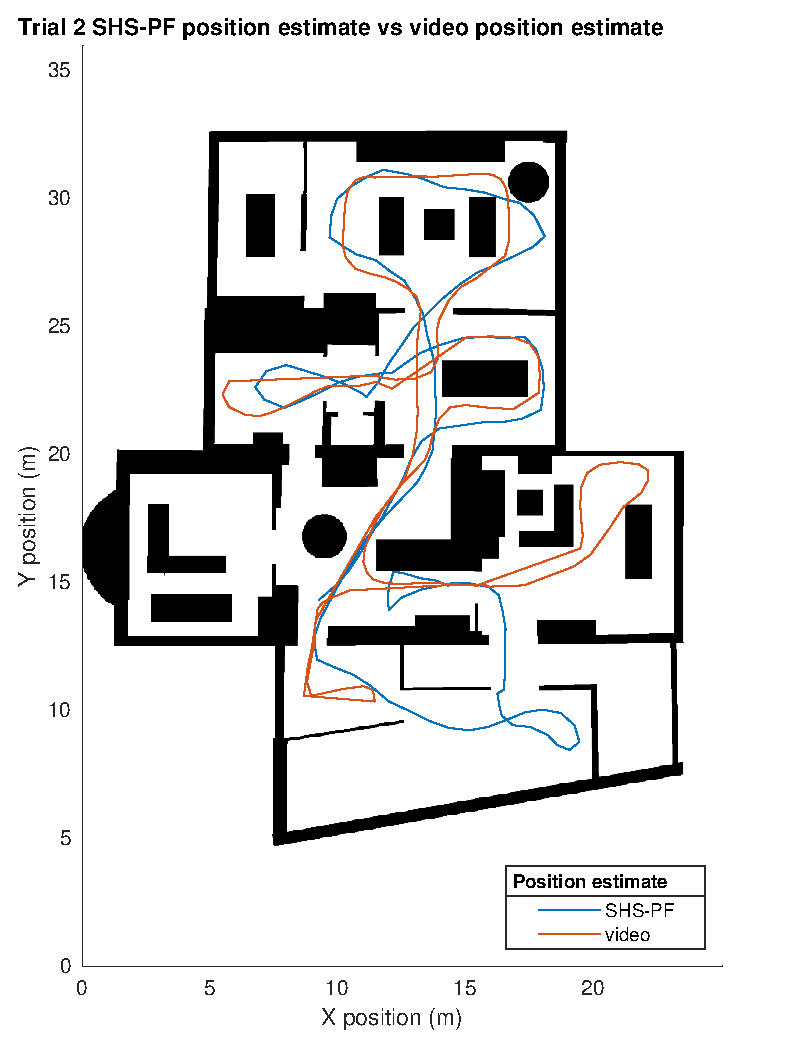
\includegraphics[width=0.95\textwidth]{images/20201129_1904_trial_2_map_1}};
			\begin{scope}[x={(image.south east)},y={(image.north west)}]
				\draw[green,ultra thick,rounded corners] (0.42,0.38) rectangle (0.37,0.4);
			\end{scope}
		\end{tikzpicture}
		\caption{Position estimate trajectory comparison. }
		\label{fig:shspf_trial2_on_map}
	\end{subfigure}
	\begin{subfigure}[t]{.45\textwidth}
		\centering
		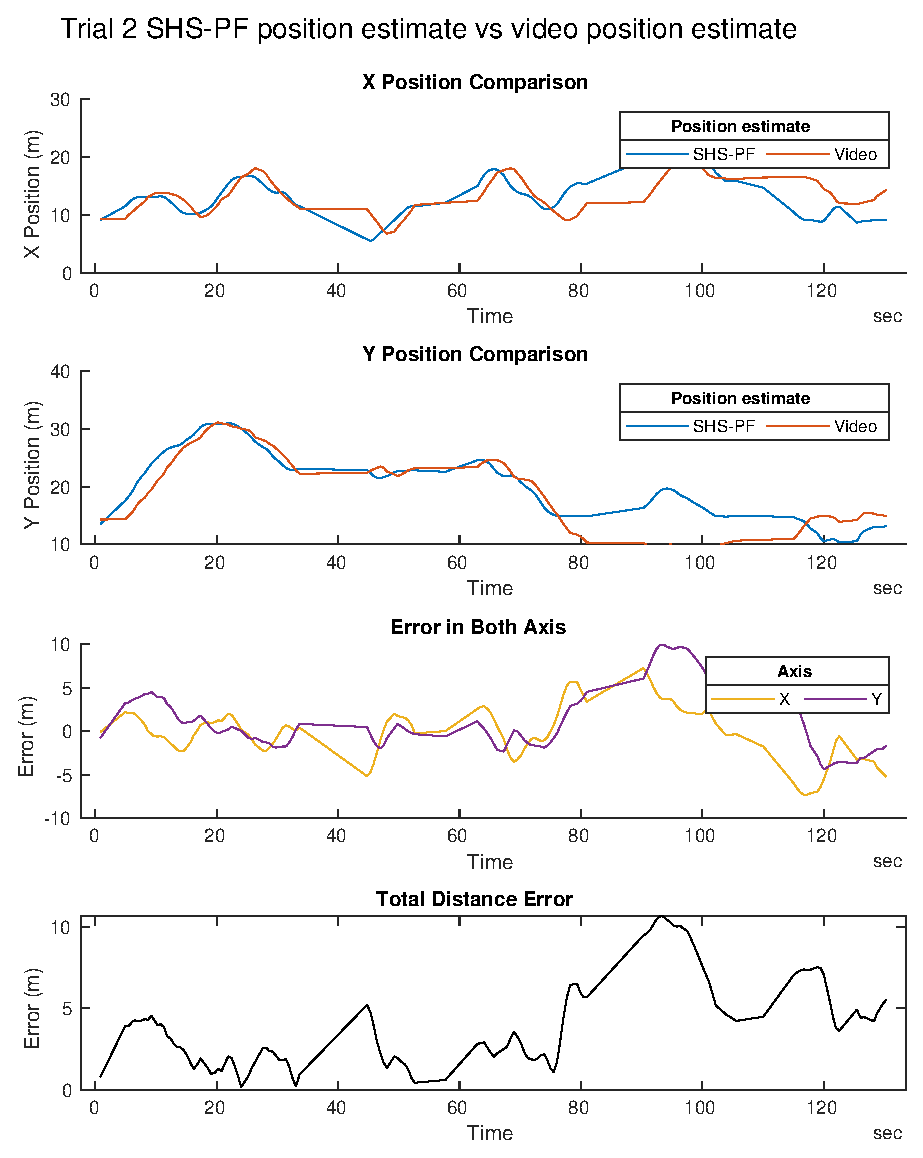
\includegraphics[width=\linewidth]{images/20201129_1904_trial_2_traj_1}
		\caption{Position estimate axis comparison.}
		\label{fig:shspf_trial2_comparison}
	\end{subfigure}
	\setlength{\belowcaptionskip}{-20pt}
	\caption{Trial 2 position comparison between SHS-PF and video position estimate. Green circled opening shows were the SHS-PF estimated to far, unable to follow the correct path, but still able to survive the run.}
	\label{fig:shspf_trial2_shs_gt_comparison}
\end{figure}

\subsection{SHS-PF with Door Interaction}
In the indoor experiment, two forms of door interaction measurement were gathered. One form was indicated manually, while the other is derived from smartwatch \ac{IMU} data and \ac{SHS} data using the activity recognition scheme of \cref{sec:method-AR}.  First, the manual situation will be treated and compared to the scenario in which the interaction are not available. Afterwards the door interactions through detection will be presented and compared with the manual case.\par


\subsubsection{SHS-PF with Manually Labeled Door Interaction}
\label{sec:results-SHS_PF_manually indicated}

Manually labeled door interactions consist of timestamps recorded manually on the smartphone to indicate the beginning of interaction with a door within the indoor environment. This is the moment when a hand makes contact with a door handle to open the door. \par 

The recorded timestamps can be used to trigger a Particle Filter door interaction measurement update. Using this method, the potential effect of activity recognition for indoor localization in the ideal case can be evaluated, since there is no chance for false positives to occur.
First, the standard deviations in the time update of the Particle Filter will be determined. Once these parameters are defined, the performance of SHS-PF with manually labeled door interaction is evaluated.

\underline{Determining Particle Filter Time Update Standard Deviations}

The same parameter sweep used for determining model standard deviations in \cref{sec:SHS-PF_without_door_interaction} is now used in the scenario of manually indicated door interactions. The parameter sweep of trial 3 can be found in \cref{fig:rmse_between_video_trajectory_andshs-pf_for_trial_3_1}, while all others can be found in \cref{sec:app-shs_pf_noise_realization}. \par
 
Using the parameter sweep results for all trials, a combination of standard deviations was chosen for the SHS-PF to use when evaluating the performance of the design. This was based on a parameter combination which for all trials resulted in all runs being completed, with all completed runs having similar RMSE values per trial. This was set at 0.14 rad for step heading standard deviation and 0.18 meters for step length standard deviation. The decision to use the same standard deviation parameters for all trials is to show how well the SHS-PF can handle \textit{all} trials with the same parameters.  \par 

For trials 4 and 5, no combination of step heading and step length standard deviations was able to generate completed particle filter runs consistently. Increasing the number of particles did not change this. In addition, using the android orientation estimate instead of the orientation estimate of \cref{sec:meth-indoor_heading_estimation} also did not give better results. This generates the hypothesis that the underlying step and heading system trajectory is not sufficient in propagating the position estimate within the spatial constraints, and that door interaction detection is not able to compensate for it. It also indicates that there is a limit to how much door interaction measurement updates can compensate for diverging SHS trajectories.  \par

\begin{figure}[H]
	\centering
	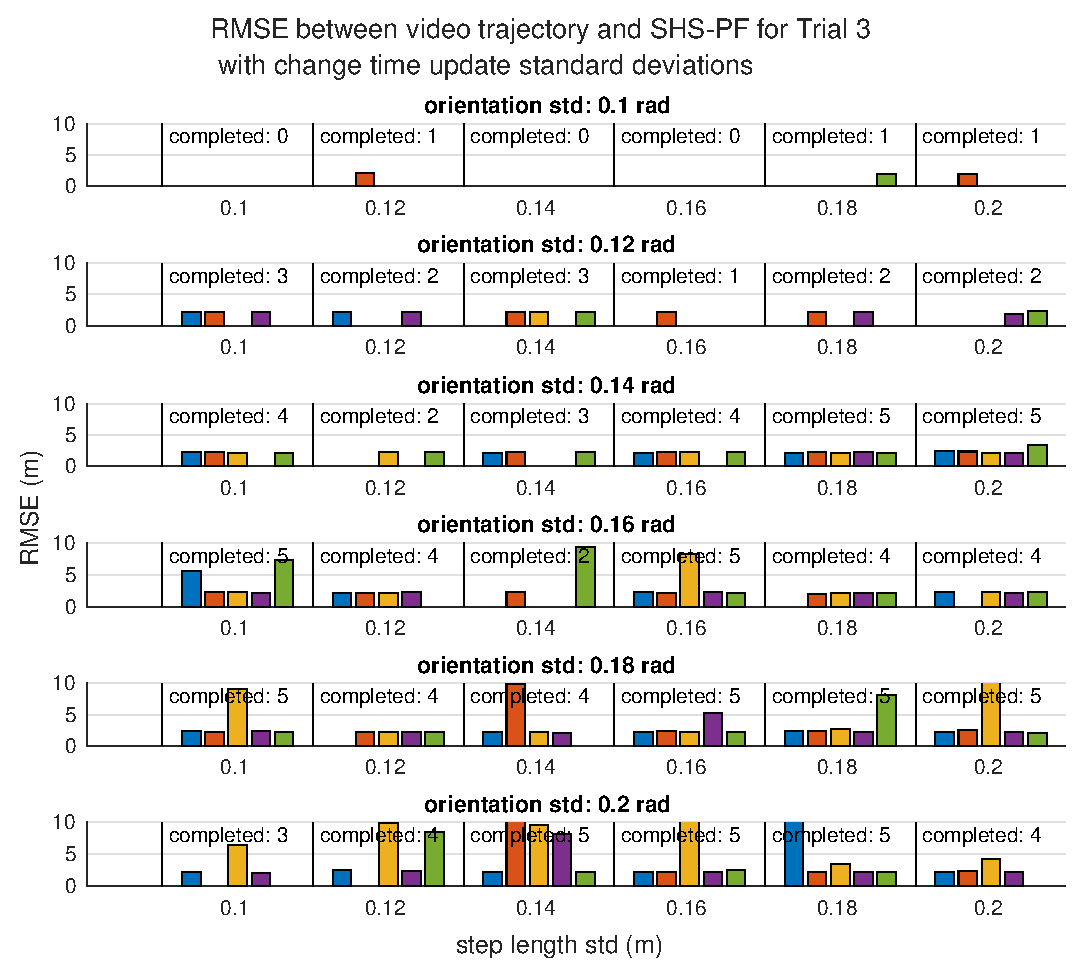
\includegraphics[width=0.85\linewidth]{images/20201201_1326_parameter_search_trial3_1}
	\caption{Parameter sweep of different standard deviation values for step heading and step length in Particle Filter time update for trial 3. The number at the top of each bar graph indicates how many Particle Filter runs were completed, and the bars show the RMSE value for each completed run between the SHS-PF estimate and the video position estimate.  }
	\label{fig:rmse_between_video_trajectory_andshs-pf_for_trial_3_1}
\end{figure}

%\underline{Determining Number of Particles}\\
%Now that the standard deviations of the particle filter time update have been found using 2000 particles, test can be performed to see what effect the number of particles has on the eventual position estimate. The results for trial 1 can be found in \cref{fig:trial1_nr_particles}, where 10 runs with an increasing number of particles was performed.  \cref{fig:trial1_nr_particles_complete} shows how many runs were completed with increasing number of particles. \cref{fig:trial1_nr_particles_RMSE} shows how the RMSE between the video trajectory and the SHS-PF position estimate changes with increasing particle filters. The same type of figures are shown in \cref{fig:trial3_nr_particles}, but then for trial 3. \par 
%
%The results in \cref{fig:trial1_nr_particles} shows that for trial 1 using 1000 particles is enough for all runs to complete the SHS trajectory. The results also show that the variance of the RMSE between the SHS-PF trajectory and the video trajectory does not change significantly as the number of particles increases. The results for trial 2 are very similar to those of trial 1, requiring only 500 particles to complete ten runs successfully, with little change in RMSE variation. The figures of trial 2 can be found in \cref{app:SHS-PF trials}.  \par
% 
%\begin{figure}[H]
%	\centering
%	\begin{subfigure}[t]{.4\textwidth}
%		\centering
%		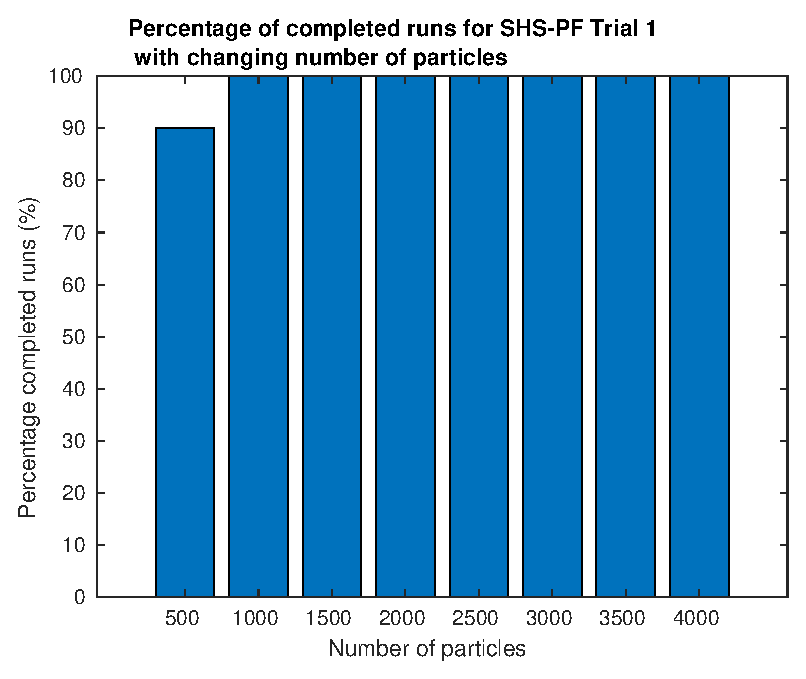
\includegraphics[width=\linewidth]{images/20201129_1147_Trial_1_nr_particles_1}
%		\caption{Percentage completed runs out of 10 runs for SHS-PF with increasing number of particles.}
%		\label{fig:trial1_nr_particles_complete}
%	\end{subfigure} \quad
%	\begin{subfigure}[t]{.4\textwidth}
%		\centering
%		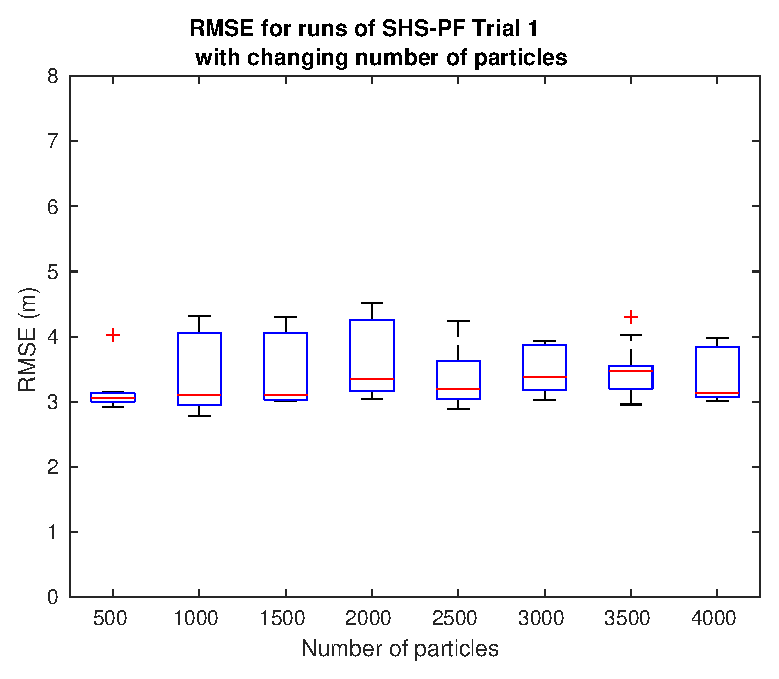
\includegraphics[width=\linewidth]{images/20201129_1154_Trial_1_RMSE_nr_particles_1}
%		\caption{RMSE between video trajectory and SHS-PF with manually indicated door interaction, with increasing number of particles}
%		\label{fig:trial1_nr_particles_RMSE}
%	\end{subfigure}
%\setlength{\belowcaptionskip}{-20pt}
%\caption{Increasing number of particles for SHS-PF in trial 1.}
%\label{fig:trial1_nr_particles}
%\end{figure}
%
%\begin{figure}[H]	
%	\centering
%	\begin{subfigure}[t]{.4\textwidth}
%		\centering
%		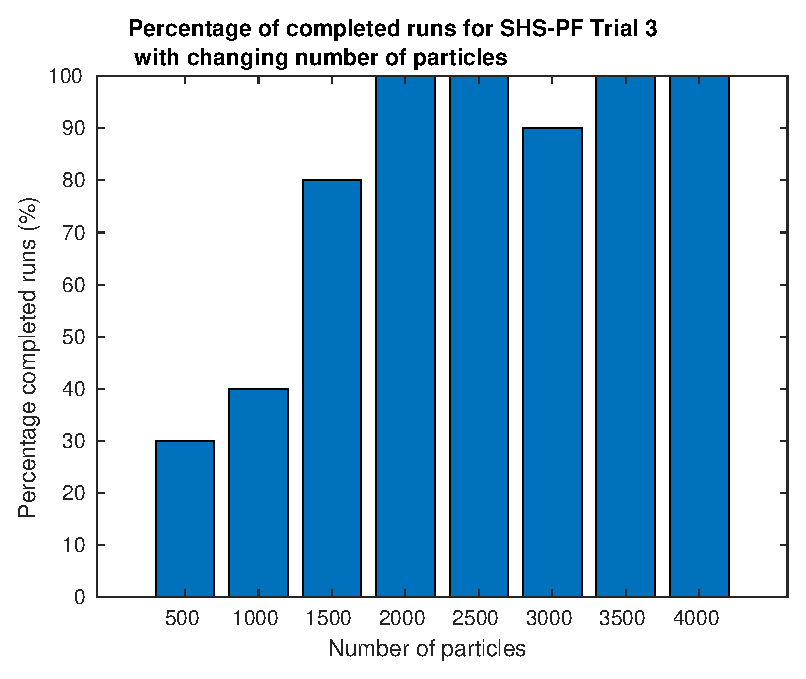
\includegraphics[width=\linewidth]{images/20201129_1147_Trial_3_nr_particles_1}
%		\caption{Percentage completed runs for SHS-PF with increasing number of particles.}
%		\label{fig:trial3_nr_particles_completed}
%	\end{subfigure} \quad
%\begin{subfigure}[t]{.4\textwidth}
%	\centering
%	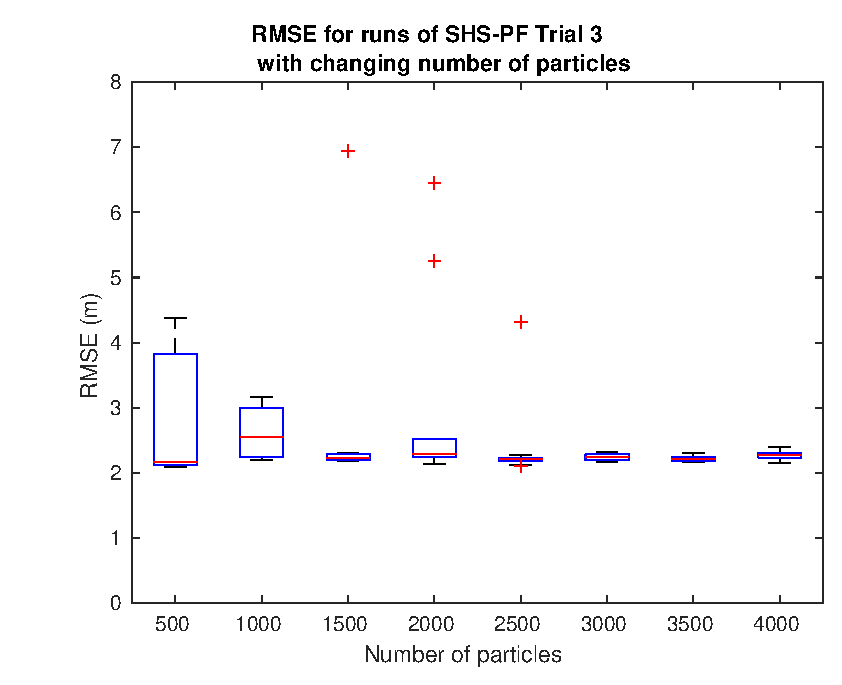
\includegraphics[width=\linewidth]{images/20201129_1154_Trial_3_RMSE_nr_particles_1}
%	\caption{RMSE between video trajectory and SHS-PF with manually indicated door interaction, with increasing number of particles}
%	\label{fig:trial3_nr_particles_RMSE}
%\end{subfigure}
%\setlength{\belowcaptionskip}{-10pt}
%\caption{Increasing number of particles for SHS-PF in trial 3.}
%\label{fig:trial3_nr_particles}
%\end{figure}
%
%The results of trial 3 in \cref{fig:trial3_nr_particles} differs from trial 1 and 2 in that the number of particles need to complete all runs successfully is larger, with one run out of 10 not completing the SHS trajectory at 3000 particles. Furthermore, the results also show that an increase in the number of particles decreases the variance of the RMSE between video trajectory and SHS-PF trajectory. This is as expected since more particles define the distribution better. %TODO check this and find a source
%\par 
%
%One hypothesis for the difference in number of particles need per trial for successful completion can be traced back to the qualitative comparison of SHS trajectory with video position estimate in \cref{sec:results-SHS_trajectories}. Here the notion of SHS trajectory quality was suggested, where higher quality follows video estimate closer. Higher quality trajectories  represent interaction with spatial constraints better, requiring only minor changes within the Particle Filter to respect the constraints completely. This would translate to less particles needed and smaller standard deviations to complete runs successfully. An example of the latter can be seen in 

\subsubsection{SHS-PF with Manually Indicated Door Interaction Performance}
Using the above results for initial parameters for model standard deviation, all trials were run through the complete SHS-PF with the manually recorded door interactions, using 2000 particles, a value determined heuristically. This was done for five runs per trial, to show reproducibility. The results can be found in \cref{fig:pf_boxplot}. The figure shows the root-mean-square error values between the SHS-PF and video position estimate per experimental trial over 5 runs. At the top of the figure, the amount of completed runs is indicated.

\begin{figure}[H]
	\centering
	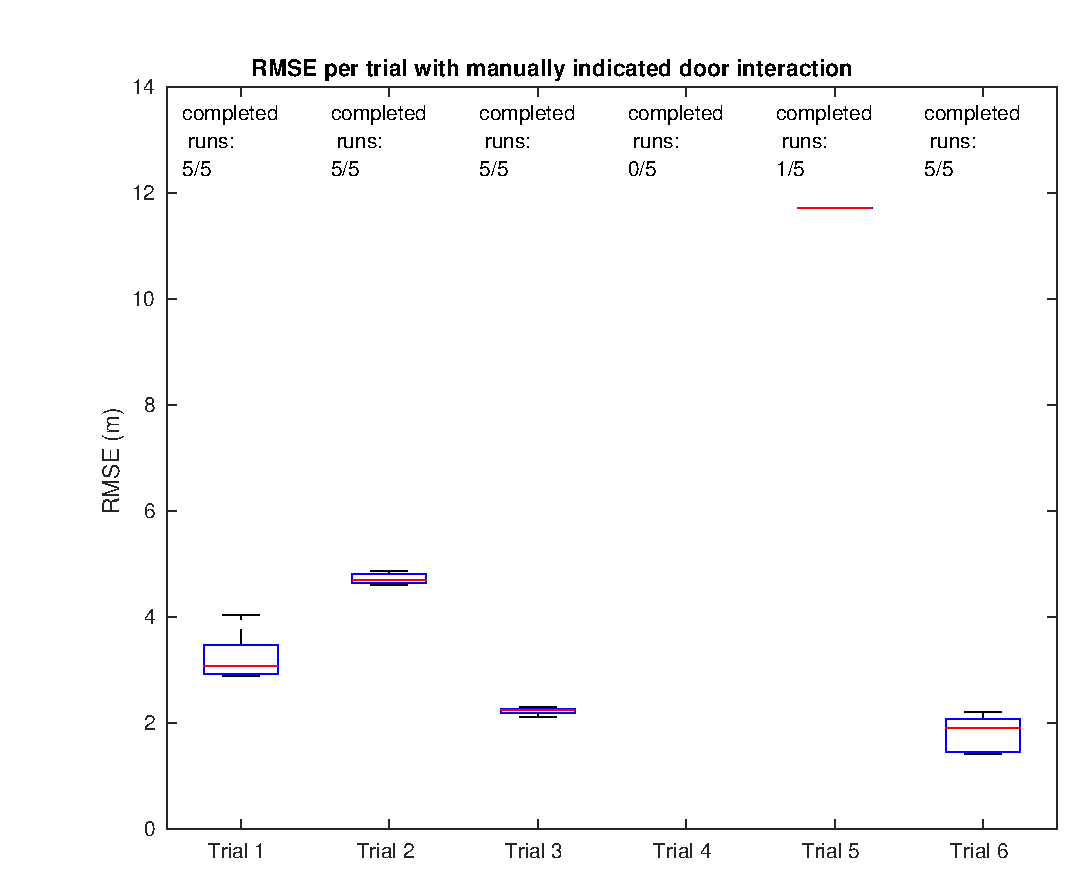
\includegraphics[width=0.7\textwidth]{images/20201201_1850_RMSE_per_trial_with_manually_indicated_door_interaction}
	\caption[Particle Filter position estimation performance with manual door interaction]{ Root-mean-square error between Particle Filter position estimate and video position estimate. Manually indicated door interactions were used for Particle Filter measurement update.}	
	\label{fig:pf_boxplot}
\end{figure}

Trials 1 and 2 do not have different RMSE values compared to those found in \cref{sec:SHS-PF_without_door_interaction}, indicating that door interaction measurement updates do not improve the position estimate of the SHS-PF for these trials. The position estimate still contain the same diverging behavior as seen before.\par 

In contrast to trials 1 and 2, the median RMSE value and spread for trials 3 and 6 are much smaller than when no door interaction was used.
Trial 3 and 6, the trajectories of which are shown in \cref{fig:shspf_trial3_shs_gt_comparison} and \cref{fig:shspf_trial6_shs_gt_comparison} respectively, are able to follow their routes much better when door interaction measurement updates are enabled. Trial 3 produces a position estimate that is very comparable to the one generated from video. Trial 6 diverges halfway through the SHS trajectory but can recuperate and generate a position estimate similar to that of the video trajectory afterwards.\par 

The results in \cref{fig:pf_boxplot} show that using the ideal form of activity recognition, where no false positives are possible, can help improve indoor localization using the design presented in \cref{chap:method}. The results of trials 1 and 3 also show that the application of activity recognition measurement updates does not always lead to improved indoor localization.

A potential reason why the Particle Filter position estimate diverges from the video trajectory is that step length estimation may be overestimating the distance traveled in some cases. This hypothesis originates from post-processing the video data, where it was qualitatively noticed that when turning a corner that the distance traveled in those steps was smaller than when walking straight. All step length testing in this thesis so far used data from test subjects that walked in a straight line, and has therefore not been affected by the phenomenon this hypothesis states.\par 

Another perspective worth considering is the infrequency with which door interaction occurs. In some trials, the time difference can amount to 50 seconds. In this time frame, the position estimate is only able to rely on the SHS trajectory and spatial constraints. This provides limited opportunities for the measurement update to occur. Enhancing the activity recognition to detect more position dependent activities, will help in counteracting diverging estimates. 
%todo door interaction help but does not gaurantee that the estimate does not diverge from the actual path. This highlights the importance of the step and heading system estimate.

%A comparison is made between the total distance traveled according to the \ac{SHS} and the video estimate. The results can be seen in \cref{fig:distance_travelled_comparison_1}. The results do not seem to support the above hypothesis, since the \ac{SHS} has underestimated the distance in all but one of the trials. While the total distance traveled is underestimated
\newpage
 
 \begin{figure}[H]
 	\centering
 	\begin{subfigure}[t]{.45\textwidth}
 		\centering
 		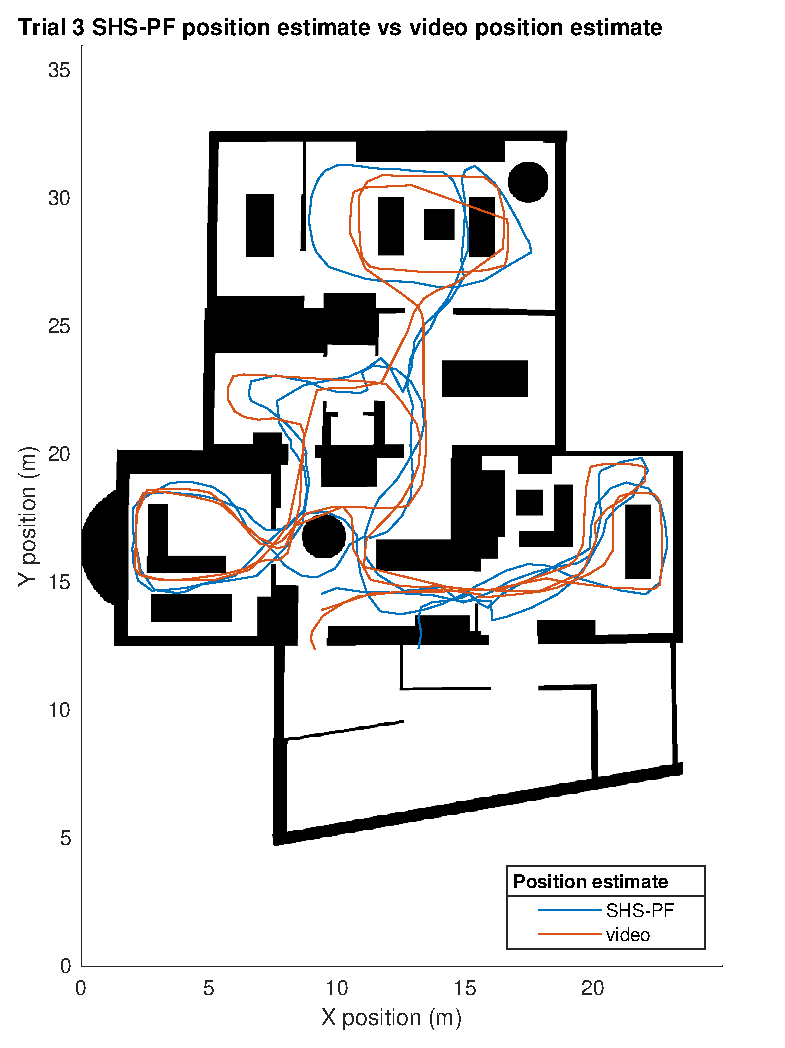
\includegraphics[width=1.02\linewidth]{images/20201129_1900_trial_3_map_1}
 		\caption{Position estimate trajectory comparison.}
 		\label{fig:shspf_trial3_on_map}
 	\end{subfigure}
 	\begin{subfigure}[t]{.45\textwidth}
 		\centering
 		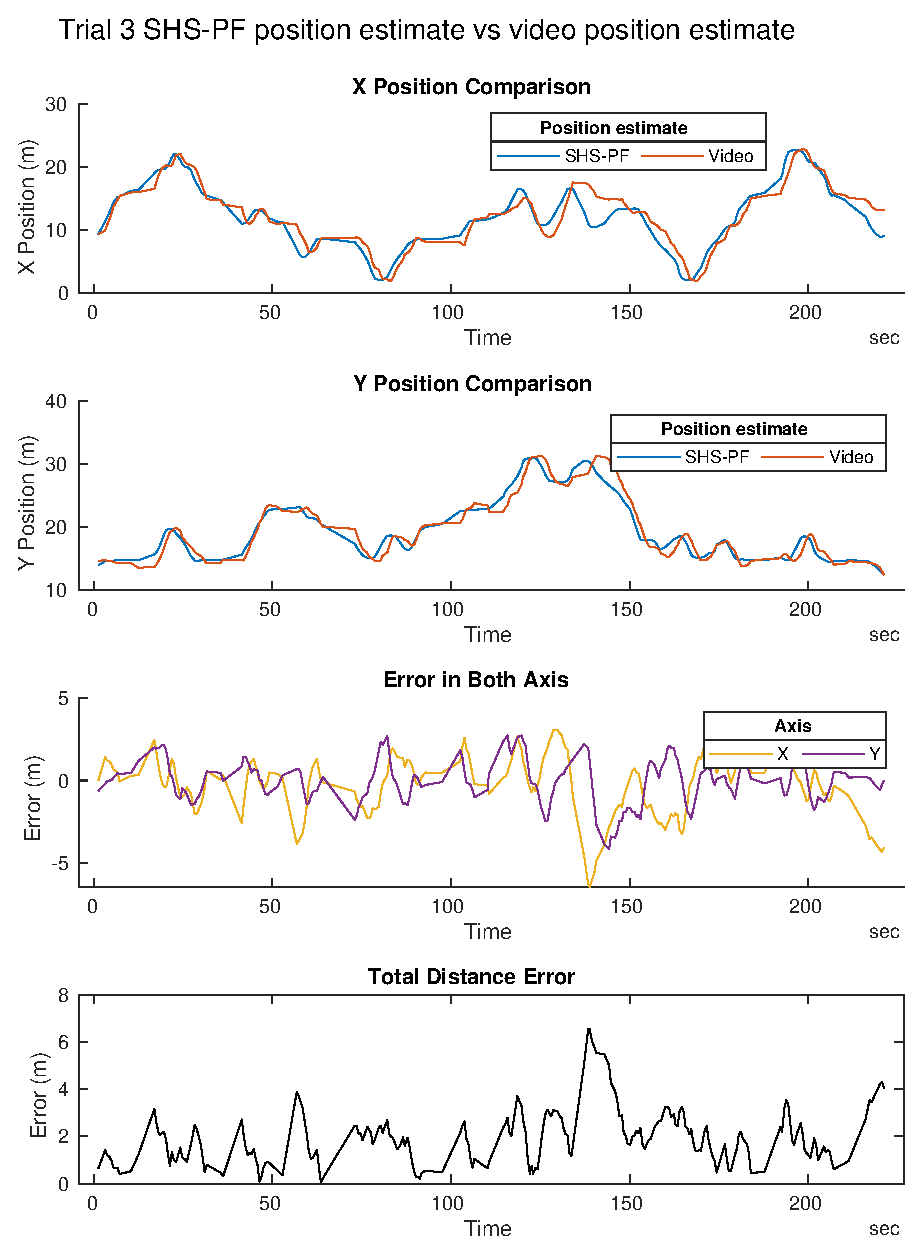
\includegraphics[width=\linewidth]{images/20201129_1900_trial_3_traj_1}
 		\caption{Position estimate axis comparison.}
 		\label{fig:shspf_trial3_comparison}
 	\end{subfigure}
 \setlength{\belowcaptionskip}{-20pt}
 	\caption{Trial 3 position comparison between SHS-PF and video position estimate. SHS-PF position estimate is shown following the video position estimate closely.}
 	\label{fig:shspf_trial3_shs_gt_comparison}
 \end{figure}
 \begin{figure}[H]
 	\centering
 	\begin{subfigure}[t]{.45\textwidth}
 		\centering
 		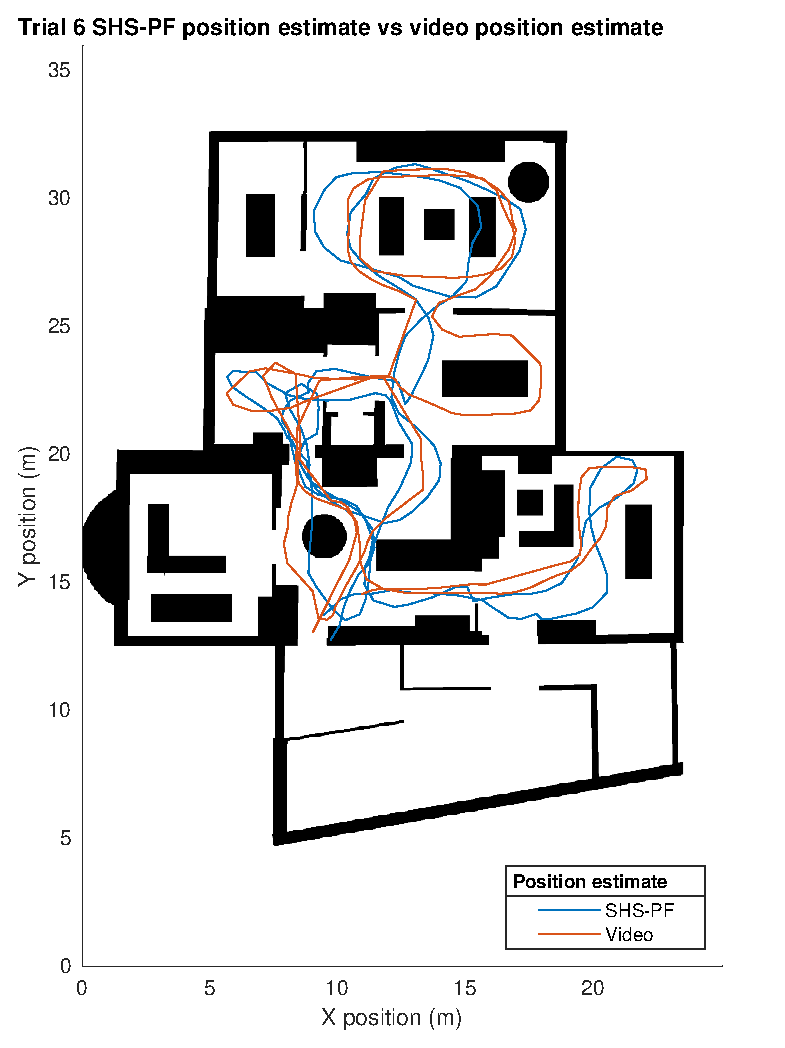
\includegraphics[width=0.95\linewidth]{images/20201129_1857_trial_6_map_1}
 		\caption{Position estimate trajectory comparison}
 		\label{fig:shspf_trial6_on_map}
 	\end{subfigure}
 	\begin{subfigure}[t]{.45\textwidth}
 		\centering
 		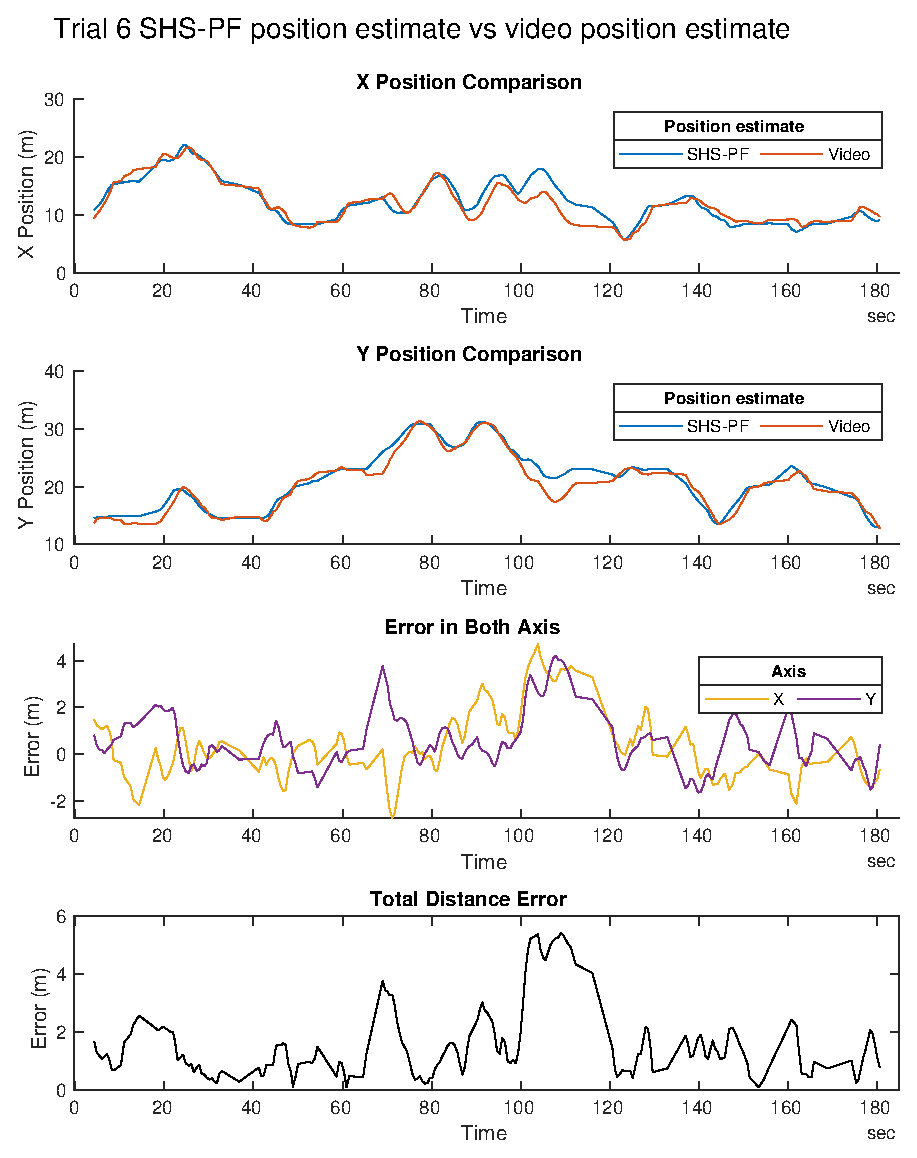
\includegraphics[width=\linewidth]{images/20201129_1858_trial_6_traj_1}
 		\caption{Position estimate axis comparison.}
 		\label{fig:shspf_trial6_comparison}
 	\end{subfigure}
 \setlength{\belowcaptionskip}{-20pt}
 	\caption{Trial 6 position comparison between SHS-PF and video position estimate. A divergence from the video estimate is shown half way through, but the correct estimate is recuperated later.  }
 	\label{fig:shspf_trial6_shs_gt_comparison}
 \end{figure}

%todo using the same standard deviation the experiment was run without door interaction results are below
%The smaller RMSE values for trial 3 and 6 can be attributed to higher particle survivability at lower model standard deviation for step heading and step length. To further highlight the effect of door interaction measurement updates, the same test as \cref{fig:pf_boxplot} was performed, where 5 runs per trial were executed with the same standard deviation values as with door interaction enable. Door interaction measurement updates were disable. All other parameters were kept the same. The results can be found in \cref{fig:pf_boxplot_no_doors}.
%
%\begin{figure}[H]
%	\centering
%	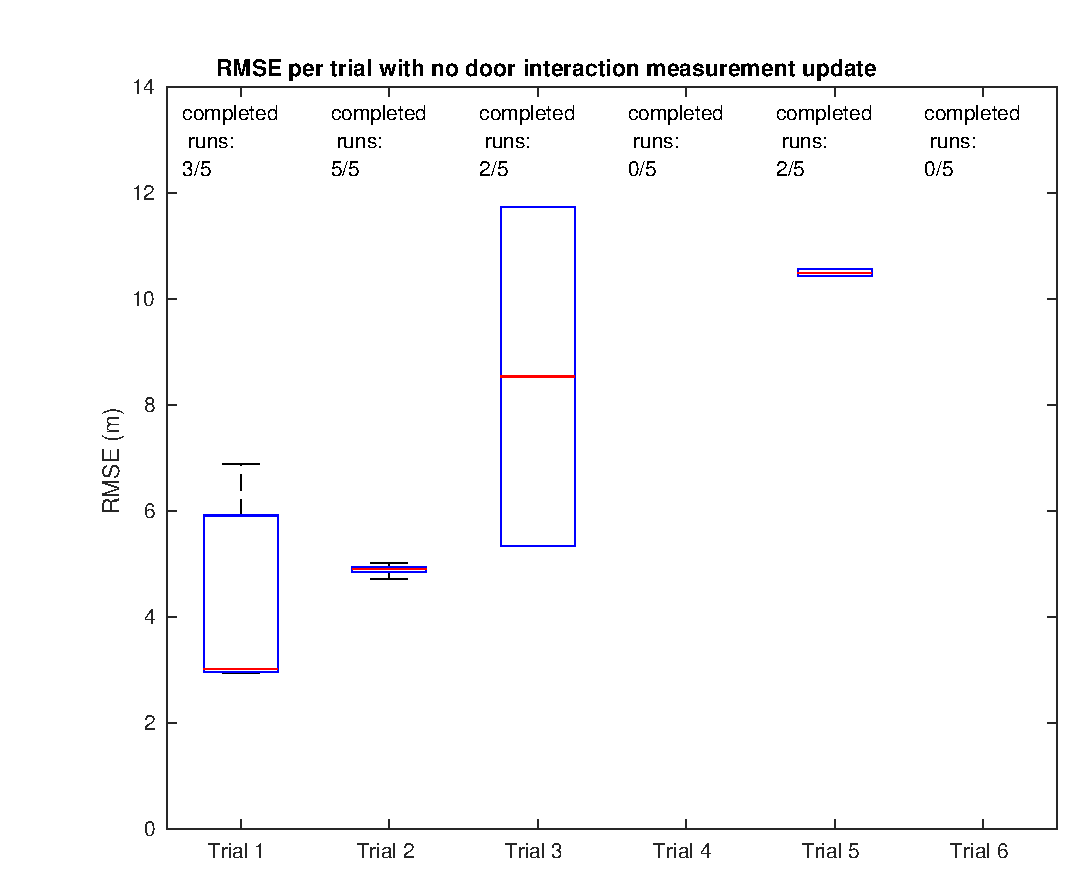
\includegraphics[width=0.7\textwidth]{images/20201201_1847_RMSE_per_trial_with_no_door_interaction_measurement_update}
%	\caption[Particle Filter position estimation performance without door interaction]{Particle Filter position estimation performance without door interaction measurement update, using same standard deviation parameters as with door interaction measurement update. 5 iterations per trial. Number under "completed runs" indicates how many runs had particles surviving for the whole \ac{SHS} trajectory.}
%	\label{fig:pf_boxplot_no_doors}
%\end{figure}
%
%%todo once the data is complete, write this section again
%The results show that for all trials except trial 2 were unable to complete all runs using the same standard deviation parameters used when door interaction measurement updates were available. This indicates that for the SHS-PF implementation constructed in this thesis, the use of activity recognition measurement updates facilitates particle survivability and therefore also the ability to complete more runs successfully. However the completed runs still have the potential to diverge from the actual path. This further highlights the importance of the step and heading system estimate. 
%
%A hypothesis for the suggested higher survivability of the particles can be related to the positioning of doors within indoor environments. Doors generally have some open space in front and behind them for easy maneuverability when passing through. Door interaction measurement updates in essence "pull" the position estimates to door location. This could allow particles to leverage the larger maneuverability within these regions, allowing the position estimate to proliferate more successfully.

% \begin{figure}[H]
% 	\centering
% 	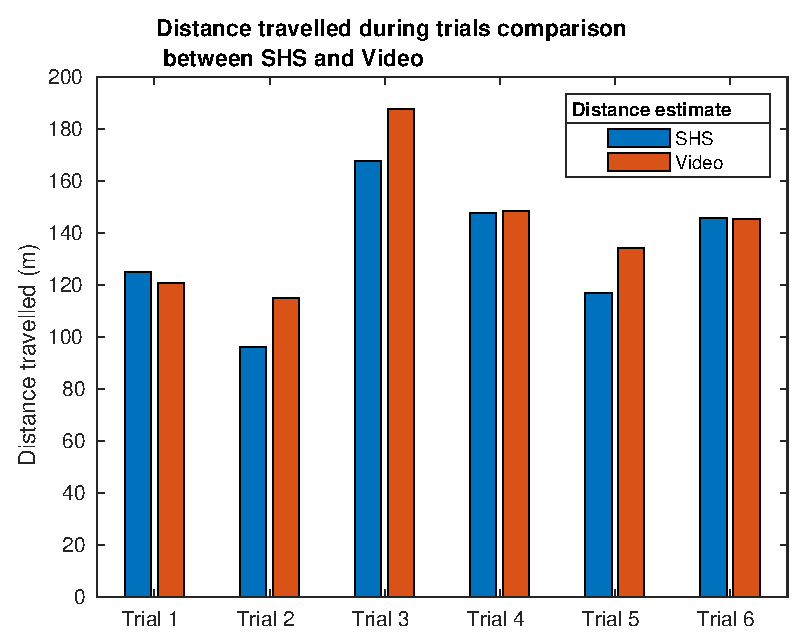
\includegraphics[width=0.7\linewidth]{images/20201129_2024_distance_travelled_comparison_1}
% 	\caption{Comparison between distance traveled estimate of SHS and video trajectory.}
% 	\label{fig:distance_travelled_comparison_1}
% \end{figure}

\subsubsection{SHS- PF with Door Interaction Detection}
So far the ideal case of door interaction detection has been treated and has shown to potentially have a positive effect compared to when they are not used. A more realistic scenario can be sketched by applying the activity recognition method outlined in Algorithm 3 on the indoor experiment data. Using these detections instead of the manually indicated ones, the results in \cref{fig:rmse_per_trial_with_activity_recognition} were generated. The standard deviation values used for the ideal case, are also used in this scenario.

\begin{figure}[H]
	\centering
	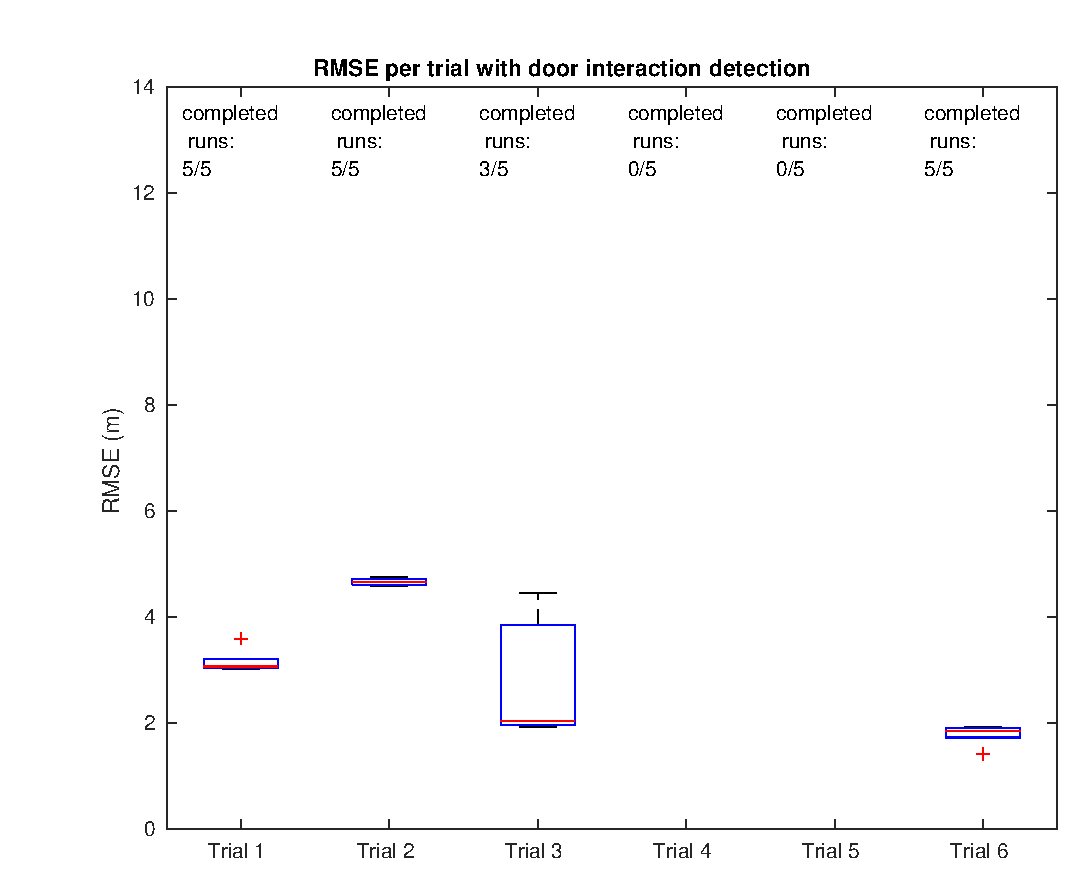
\includegraphics[width=0.7\linewidth]{images/20201201_1851_RMSE_per_trial_with_door_interaction_detection}
	\caption[Particle Filter position estimation performance with door interaction]{Particle filter position estimation root mean square error compared to rough video generated estimate using detected door interactions.}
	\label{fig:rmse_per_trial_with_activity_recognition}
\end{figure}

Trials 1,2 and 6 show similar results as when manually indicated door interactions are used, as shown in \cref{fig:pf_boxplot}. Similar RMSE values to the manually indicated door interactions can also be noticed. Also, the inability to complete all runs for trials 5 and 6 is still present. \par 

In contrast trial 3 is unable to complete all runs, with the completed iterations leading to larger RMSE values than with manually indicated interactions. The reason for this can be seen in \cref{fig:video_traj_trial3_door_detect_vs_manual_1}. In this plot, the position estimate from the video can be seen as the blue line. The markers on the path indicate the position at the time point in the video trajectory when door interactions are detected and indicated manually; green and red respectively. The plot shows clear clusters of detections and manually indicated points. There is however one outlier at a  x position of 10.5 meters and y position of 27.6 meters. This point is clearly not placed close to door interaction clusters, and can therefore be labeled a false positive. \par 

This false positive can also be seen in \cref{fig:trial_3_door_interaction_detection_using_smartwatch1}, where the smartwatch accelerometer data per axis is shown. The vertical lines represent manually indicated interaction and the start of door interaction detection sections. The red dots represent accelerometer samples that meet the threshold requirements set for door detection in \cref{sec:method-AR}. The detection at 142 seconds is what caused the false positive.\par 

Replaying the video for this trial at this time point, the test subject is seen interacting with the smartwatch with the hand holding the smartphone, attempting to check whether smartphone IMU recording is functioning properly. This action unintentionally performed a movement that meets the threshold requirements for a door interaction detection, triggering a detection. \par 

\begin{figure}[H]
	\centering
	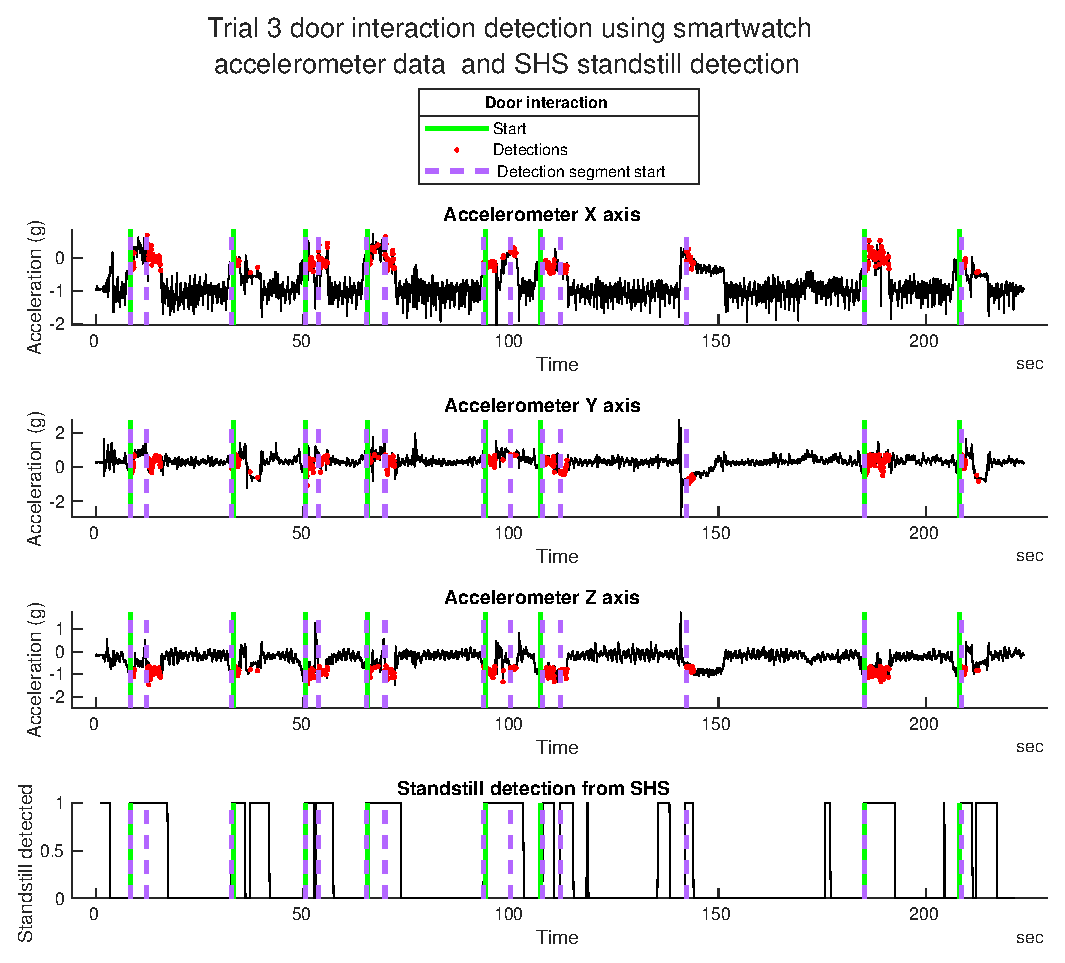
\includegraphics[width=0.9\linewidth]{images/20201201_1505_Trial_3_door_interaction_detection_using_smartwatch_1}
	\setlength{\belowcaptionskip}{-10pt}
	\caption{Trial 3 door interaction detection using smartwatch accelerometer data. The detection at 142 seconds is a false positive.}
	\label{fig:trial_3_door_interaction_detection_using_smartwatch1}
\end{figure}

The false positive door interaction detection in trial 3 highlights some of the shortcomings with the indoor localization implementation presented in this thesis. It indicates that falsely triggered Particle Filter measurement updates can cause position estimates to diverge and potentially render it unable to generate a position estimate for all SHS time steps. It highlights the robustness need from activity recognition for the implementation presented in this thesis.

\begin{figure}[H]
	\centering
	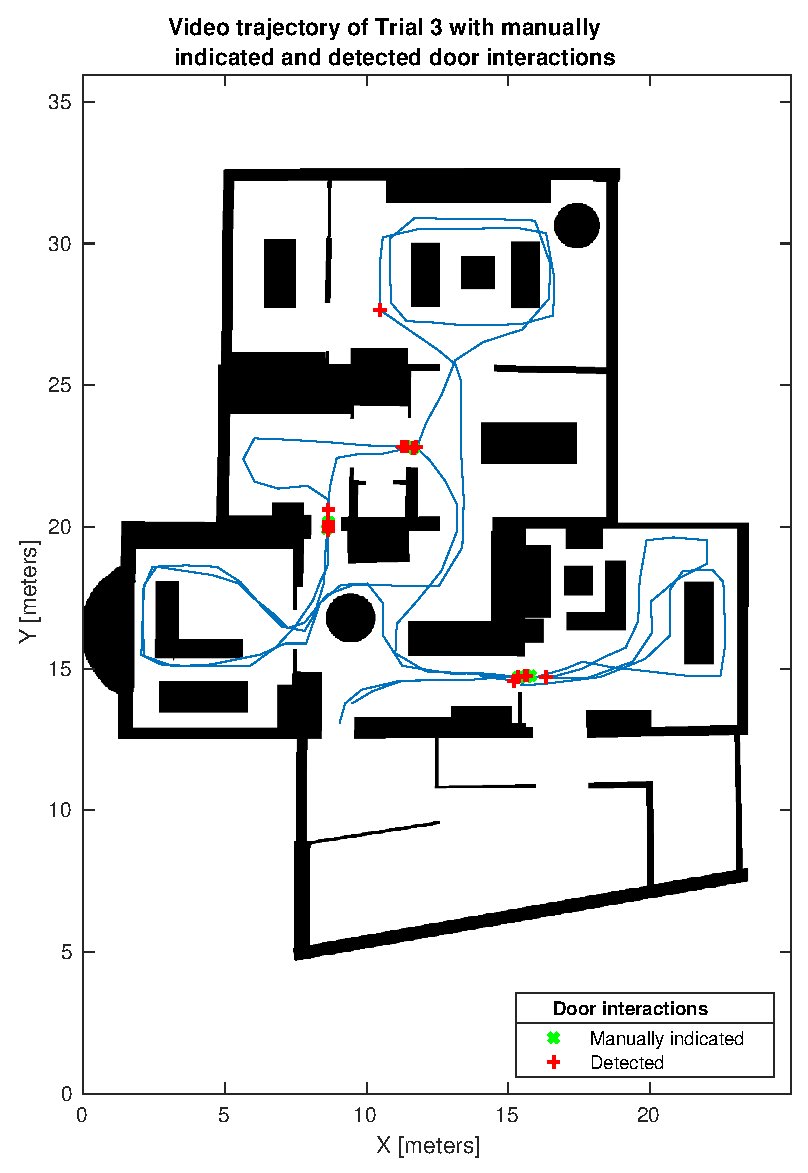
\includegraphics[width=0.7\linewidth]{images/20201129_2330_video_traj_Trial_3_door_detect_vs_manual_1}
	\setlength{\belowcaptionskip}{-10pt}
	\caption{position estimate from video estimate with markers on the path indicating the position at the time point in the video trajectory when door interactions are detected and indicated manually.}
	\label{fig:video_traj_trial3_door_detect_vs_manual_1}
\end{figure}
 
 
 
 